\documentclass[twoside]{book}

% Packages required by doxygen
\usepackage{calc}
\usepackage{doxygen}
\usepackage{graphicx}
\usepackage[utf8]{inputenc}
\usepackage{makeidx}
\usepackage{multicol}
\usepackage{multirow}
\usepackage{textcomp}
\usepackage[table]{xcolor}

% Font selection
\usepackage[T1]{fontenc}
\usepackage{mathptmx}
\usepackage[scaled=.90]{helvet}
\usepackage{courier}
\usepackage{amssymb}
\usepackage{sectsty}
\renewcommand{\familydefault}{\sfdefault}
\allsectionsfont{%
  \fontseries{bc}\selectfont%
  \color{darkgray}%
}
\renewcommand{\DoxyLabelFont}{%
  \fontseries{bc}\selectfont%
  \color{darkgray}%
}

% Page & text layout
\usepackage{geometry}
\geometry{%
  a4paper,%
  top=2.5cm,%
  bottom=2.5cm,%
  left=2.5cm,%
  right=2.5cm%
}
\tolerance=750
\hfuzz=15pt
\hbadness=750
\setlength{\emergencystretch}{15pt}
\setlength{\parindent}{0cm}
\setlength{\parskip}{0.2cm}
\makeatletter
\renewcommand{\paragraph}{%
  \@startsection{paragraph}{4}{0ex}{-1.0ex}{1.0ex}{%
    \normalfont\normalsize\bfseries\SS@parafont%
  }%
}
\renewcommand{\subparagraph}{%
  \@startsection{subparagraph}{5}{0ex}{-1.0ex}{1.0ex}{%
    \normalfont\normalsize\bfseries\SS@subparafont%
  }%
}
\makeatother

% Headers & footers
\usepackage{fancyhdr}
\pagestyle{fancyplain}
\fancyhead[LE]{\fancyplain{}{\bfseries\thepage}}
\fancyhead[CE]{\fancyplain{}{}}
\fancyhead[RE]{\fancyplain{}{\bfseries\leftmark}}
\fancyhead[LO]{\fancyplain{}{\bfseries\rightmark}}
\fancyhead[CO]{\fancyplain{}{}}
\fancyhead[RO]{\fancyplain{}{\bfseries\thepage}}
\fancyfoot[LE]{\fancyplain{}{}}
\fancyfoot[CE]{\fancyplain{}{}}
\fancyfoot[RE]{\fancyplain{}{\bfseries\scriptsize Generated on Wed Dec 23 2015 09\-:32\-:50 for U\-S\-A\-R\-T by Doxygen }}
\fancyfoot[LO]{\fancyplain{}{\bfseries\scriptsize Generated on Wed Dec 23 2015 09\-:32\-:50 for U\-S\-A\-R\-T by Doxygen }}
\fancyfoot[CO]{\fancyplain{}{}}
\fancyfoot[RO]{\fancyplain{}{}}
\renewcommand{\footrulewidth}{0.4pt}
\renewcommand{\chaptermark}[1]{%
  \markboth{#1}{}%
}
\renewcommand{\sectionmark}[1]{%
  \markright{\thesection\ #1}%
}

% Indices & bibliography
\usepackage{natbib}
\usepackage[titles]{tocloft}
\setcounter{tocdepth}{3}
\setcounter{secnumdepth}{5}
\makeindex

% Hyperlinks (required, but should be loaded last)
\usepackage{ifpdf}
\ifpdf
  \usepackage[pdftex,pagebackref=true]{hyperref}
\else
  \usepackage[ps2pdf,pagebackref=true]{hyperref}
\fi
\hypersetup{%
  colorlinks=true,%
  linkcolor=blue,%
  citecolor=blue,%
  unicode%
}

% Custom commands
\newcommand{\clearemptydoublepage}{%
  \newpage{\pagestyle{empty}\cleardoublepage}%
}


%===== C O N T E N T S =====

\begin{document}

% Titlepage & ToC
\hypersetup{pageanchor=false}
\pagenumbering{roman}
\begin{titlepage}
\vspace*{7cm}
\begin{center}%
{\Large U\-S\-A\-R\-T \\[1ex]\large 00001 }\\
\vspace*{1cm}
{\large Generated by Doxygen 1.8.6}\\
\vspace*{0.5cm}
{\small Wed Dec 23 2015 09:32:50}\\
\end{center}
\end{titlepage}
\clearemptydoublepage
\tableofcontents
\clearemptydoublepage
\pagenumbering{arabic}
\hypersetup{pageanchor=true}

%--- Begin generated contents ---
\chapter{Todo List}
\label{todo}
\hypertarget{todo}{}

\begin{DoxyRefList}
\item[\label{todo__todo000001}%
\hypertarget{todo__todo000001}{}%
Member \hyperlink{_f_i_f_o_8h_a8328a1725cddf8c3b62939cb86037b9c}{F\-I\-F\-O\-\_\-\-Read} (uint8\-\_\-t $\ast$output\-Data\-Pointer)]Remove me 
\end{DoxyRefList}
\chapter{Class Index}
\section{Class List}
Here are the classes, structs, unions and interfaces with brief descriptions\-:\begin{DoxyCompactList}
\item\contentsline{section}{\hyperlink{union_data_converter}{Data\-Converter} \\*Define the union type used to convert between types }{\pageref{union_data_converter}}{}
\item\contentsline{section}{\hyperlink{struct_list_of_parameter_structure_type}{List\-Of\-Parameter\-Structure\-Type} \\*Defines the list of parameter data structure }{\pageref{struct_list_of_parameter_structure_type}}{}
\item\contentsline{section}{\hyperlink{struct_param_structure_type}{Param\-Structure\-Type} \\*Defines the parameter data type }{\pageref{struct_param_structure_type}}{}
\item\contentsline{section}{\hyperlink{struct_serial_interface}{Serial\-Interface} \\*Define the standard serial interface }{\pageref{struct_serial_interface}}{}
\item\contentsline{section}{\hyperlink{struct_tick_type}{Tick\-Type} \\*Defines a non-\/blocking delay data type }{\pageref{struct_tick_type}}{}
\end{DoxyCompactList}

\chapter{File Index}
\section{File List}
Here is a list of all documented files with brief descriptions\-:\begin{DoxyCompactList}
\item\contentsline{section}{\hyperlink{common_8h}{common.\-h} \\*Holds all common code definitions }{\pageref{common_8h}}{}
\item\contentsline{section}{\hyperlink{_f_i_f_o_8c}{F\-I\-F\-O.\-c} \\*This is our F\-I\-F\-O library }{\pageref{_f_i_f_o_8c}}{}
\item\contentsline{section}{\hyperlink{_f_i_f_o_8h}{F\-I\-F\-O.\-h} }{\pageref{_f_i_f_o_8h}}{}
\item\contentsline{section}{\hyperlink{led_8c}{led.\-c} \\*This is the L\-E\-D hardware interface layer }{\pageref{led_8c}}{}
\item\contentsline{section}{\hyperlink{led_8h}{led.\-h} }{\pageref{led_8h}}{}
\item\contentsline{section}{\hyperlink{main_8c}{main.\-c} \\*This is the main program code }{\pageref{main_8c}}{}
\item\contentsline{section}{\hyperlink{_serial_structure_8h}{Serial\-Structure.\-h} \\*Define the serial interface layer structure }{\pageref{_serial_structure_8h}}{}
\item\contentsline{section}{{\bfseries stm32f0xx\-\_\-conf.\-h} }{\pageref{stm32f0xx__conf_8h}}{}
\item\contentsline{section}{\hyperlink{tick_8c}{tick.\-c} \\*Implements mili-\/second tick counter }{\pageref{tick_8c}}{}
\item\contentsline{section}{\hyperlink{tick_8h}{tick.\-h} }{\pageref{tick_8h}}{}
\item\contentsline{section}{\hyperlink{usart2_8c}{usart2.\-c} \\*S\-T\-M32 serial2 M\-C\-U hardware interface layer. to maintain code portability, the hardware related code is split from the main logic }{\pageref{usart2_8c}}{}
\item\contentsline{section}{\hyperlink{usart2_8h}{usart2.\-h} }{\pageref{usart2_8h}}{}
\end{DoxyCompactList}

\chapter{Class Documentation}
\hypertarget{union_data_converter}{\section{Data\-Converter Union Reference}
\label{union_data_converter}\index{Data\-Converter@{Data\-Converter}}
}


define the union type used to convert between types.  




{\ttfamily \#include $<$common.\-h$>$}

\subsection*{Public Attributes}
\begin{DoxyCompactItemize}
\item 
\hypertarget{union_data_converter_ae9dce194bf800c0ea89942da406dc525}{long double \hyperlink{union_data_converter_ae9dce194bf800c0ea89942da406dc525}{d34\-\_\-t}}\label{union_data_converter_ae9dce194bf800c0ea89942da406dc525}

\begin{DoxyCompactList}\small\item\em 64bit I\-E\-E\-E floating point number \end{DoxyCompactList}\item 
\hypertarget{union_data_converter_ac99b9f7c8af24916e3b7993c1928b4f2}{float \hyperlink{union_data_converter_ac99b9f7c8af24916e3b7993c1928b4f2}{f32\-\_\-t} \mbox{[}2\mbox{]}}\label{union_data_converter_ac99b9f7c8af24916e3b7993c1928b4f2}

\begin{DoxyCompactList}\small\item\em 32bit I\-E\-E\-E float point number \end{DoxyCompactList}\item 
\hypertarget{union_data_converter_a20845be2f89b1012e3942dca4c5fa117}{uint32\-\_\-t \hyperlink{union_data_converter_a20845be2f89b1012e3942dca4c5fa117}{ui32\-\_\-t} \mbox{[}2\mbox{]}}\label{union_data_converter_a20845be2f89b1012e3942dca4c5fa117}

\begin{DoxyCompactList}\small\item\em unsigned 32bit. \end{DoxyCompactList}\item 
\hypertarget{union_data_converter_a0cf5f8f2f3ba3f3e1a1c44a21248d910}{int32\-\_\-t \hyperlink{union_data_converter_a0cf5f8f2f3ba3f3e1a1c44a21248d910}{i32\-\_\-t} \mbox{[}2\mbox{]}}\label{union_data_converter_a0cf5f8f2f3ba3f3e1a1c44a21248d910}

\begin{DoxyCompactList}\small\item\em signed 32bit. \end{DoxyCompactList}\item 
\hypertarget{union_data_converter_ae96584b1dad4adab583405970fc89137}{uint16\-\_\-t \hyperlink{union_data_converter_ae96584b1dad4adab583405970fc89137}{ui16\-\_\-t} \mbox{[}4\mbox{]}}\label{union_data_converter_ae96584b1dad4adab583405970fc89137}

\begin{DoxyCompactList}\small\item\em unsigned 16bit. \end{DoxyCompactList}\item 
\hypertarget{union_data_converter_ad566a31830c516b559b9a3758ad39d82}{int16\-\_\-t \hyperlink{union_data_converter_ad566a31830c516b559b9a3758ad39d82}{i16\-\_\-t} \mbox{[}4\mbox{]}}\label{union_data_converter_ad566a31830c516b559b9a3758ad39d82}

\begin{DoxyCompactList}\small\item\em signed 16bit. \end{DoxyCompactList}\item 
\hypertarget{union_data_converter_a6576e61c59bc9d4e1b54f881fe5acdd4}{uint8\-\_\-t \hyperlink{union_data_converter_a6576e61c59bc9d4e1b54f881fe5acdd4}{ui8\-\_\-t} \mbox{[}8\mbox{]}}\label{union_data_converter_a6576e61c59bc9d4e1b54f881fe5acdd4}

\begin{DoxyCompactList}\small\item\em unsigned 8bit. \end{DoxyCompactList}\item 
\hypertarget{union_data_converter_a0b79bc0f32d5bc76317f226dfc1a0325}{int8\-\_\-t \hyperlink{union_data_converter_a0b79bc0f32d5bc76317f226dfc1a0325}{i8\-\_\-t} \mbox{[}8\mbox{]}}\label{union_data_converter_a0b79bc0f32d5bc76317f226dfc1a0325}

\begin{DoxyCompactList}\small\item\em singed 8bit. \end{DoxyCompactList}\end{DoxyCompactItemize}


\subsection{Detailed Description}
define the union type used to convert between types. 

The documentation for this union was generated from the following file\-:\begin{DoxyCompactItemize}
\item 
\hyperlink{common_8h}{common.\-h}\end{DoxyCompactItemize}

\hypertarget{struct_list_of_parameter_structure_type}{\section{List\-Of\-Parameter\-Structure\-Type Struct Reference}
\label{struct_list_of_parameter_structure_type}\index{List\-Of\-Parameter\-Structure\-Type@{List\-Of\-Parameter\-Structure\-Type}}
}


Defines the list of parameter data structure.  




Collaboration diagram for List\-Of\-Parameter\-Structure\-Type\-:\nopagebreak
\begin{figure}[H]
\begin{center}
\leavevmode
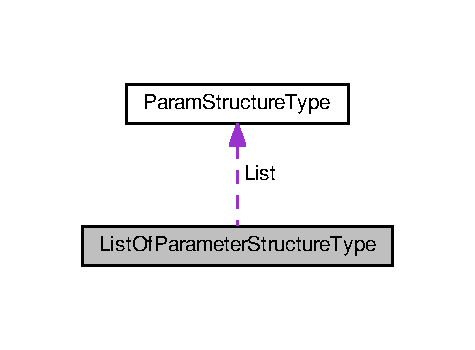
\includegraphics[width=228pt]{struct_list_of_parameter_structure_type__coll__graph}
\end{center}
\end{figure}
\subsection*{Public Attributes}
\begin{DoxyCompactItemize}
\item 
uint32\-\_\-t \hyperlink{struct_list_of_parameter_structure_type_a10041e965575f7a0a57158d2cc52b9e7}{Number\-Of\-Parameter}
\begin{DoxyCompactList}\small\item\em used to keep track of the number of parameter we haver \end{DoxyCompactList}\item 
\hyperlink{struct_param_structure_type}{Param\-Structure\-Type} \hyperlink{struct_list_of_parameter_structure_type_a9079f3b980c4a6f735367b19c375e6f9}{List} \mbox{[}10\mbox{]}
\begin{DoxyCompactList}\small\item\em hold the parameter \end{DoxyCompactList}\end{DoxyCompactItemize}


\subsection{Detailed Description}
Defines the list of parameter data structure. 

\subsection{Member Data Documentation}
\hypertarget{struct_list_of_parameter_structure_type_a9079f3b980c4a6f735367b19c375e6f9}{\index{List\-Of\-Parameter\-Structure\-Type@{List\-Of\-Parameter\-Structure\-Type}!List@{List}}
\index{List@{List}!ListOfParameterStructureType@{List\-Of\-Parameter\-Structure\-Type}}
\subsubsection[{List}]{\setlength{\rightskip}{0pt plus 5cm}{\bf Param\-Structure\-Type} List\-Of\-Parameter\-Structure\-Type\-::\-List\mbox{[}10\mbox{]}}}\label{struct_list_of_parameter_structure_type_a9079f3b980c4a6f735367b19c375e6f9}


hold the parameter 

\hypertarget{struct_list_of_parameter_structure_type_a10041e965575f7a0a57158d2cc52b9e7}{\index{List\-Of\-Parameter\-Structure\-Type@{List\-Of\-Parameter\-Structure\-Type}!Number\-Of\-Parameter@{Number\-Of\-Parameter}}
\index{Number\-Of\-Parameter@{Number\-Of\-Parameter}!ListOfParameterStructureType@{List\-Of\-Parameter\-Structure\-Type}}
\subsubsection[{Number\-Of\-Parameter}]{\setlength{\rightskip}{0pt plus 5cm}uint32\-\_\-t List\-Of\-Parameter\-Structure\-Type\-::\-Number\-Of\-Parameter}}\label{struct_list_of_parameter_structure_type_a10041e965575f7a0a57158d2cc52b9e7}


used to keep track of the number of parameter we haver 



The documentation for this struct was generated from the following file\-:\begin{DoxyCompactItemize}
\item 
\hyperlink{_terminal_8c}{Terminal.\-c}\end{DoxyCompactItemize}

\hypertarget{struct_param_structure_type}{\section{Param\-Structure\-Type Struct Reference}
\label{struct_param_structure_type}\index{Param\-Structure\-Type@{Param\-Structure\-Type}}
}


Defines the parameter data type.  


\subsection*{Public Attributes}
\begin{DoxyCompactItemize}
\item 
uint8\-\_\-t \hyperlink{struct_param_structure_type_a07c3f655760942fd5b06c97ff9deea4a}{Type}
\begin{DoxyCompactList}\small\item\em Parameter data type. S = command, U = integer. \end{DoxyCompactList}\item 
uint32\-\_\-t \hyperlink{struct_param_structure_type_a6804a54620bdeec3aee9a58941fef762}{Value}
\begin{DoxyCompactList}\small\item\em parameter data \end{DoxyCompactList}\end{DoxyCompactItemize}


\subsection{Detailed Description}
Defines the parameter data type. 

\subsection{Member Data Documentation}
\hypertarget{struct_param_structure_type_a07c3f655760942fd5b06c97ff9deea4a}{\index{Param\-Structure\-Type@{Param\-Structure\-Type}!Type@{Type}}
\index{Type@{Type}!ParamStructureType@{Param\-Structure\-Type}}
\subsubsection[{Type}]{\setlength{\rightskip}{0pt plus 5cm}uint8\-\_\-t Param\-Structure\-Type\-::\-Type}}\label{struct_param_structure_type_a07c3f655760942fd5b06c97ff9deea4a}


Parameter data type. S = command, U = integer. 

\hypertarget{struct_param_structure_type_a6804a54620bdeec3aee9a58941fef762}{\index{Param\-Structure\-Type@{Param\-Structure\-Type}!Value@{Value}}
\index{Value@{Value}!ParamStructureType@{Param\-Structure\-Type}}
\subsubsection[{Value}]{\setlength{\rightskip}{0pt plus 5cm}uint32\-\_\-t Param\-Structure\-Type\-::\-Value}}\label{struct_param_structure_type_a6804a54620bdeec3aee9a58941fef762}


parameter data 



The documentation for this struct was generated from the following file\-:\begin{DoxyCompactItemize}
\item 
\hyperlink{_terminal_8c}{Terminal.\-c}\end{DoxyCompactItemize}

\hypertarget{struct_serial_interface}{\section{Serial\-Interface Struct Reference}
\label{struct_serial_interface}\index{Serial\-Interface@{Serial\-Interface}}
}


define the standard serial interface  




{\ttfamily \#include $<$Serial\-Structure.\-h$>$}

\subsection*{Public Attributes}
\begin{DoxyCompactItemize}
\item 
\hypertarget{struct_serial_interface_aa12245208003c78ea024ad24f9d84f2a}{uint\-\_\-fast8\-\_\-t($\ast$ \hyperlink{struct_serial_interface_aa12245208003c78ea024ad24f9d84f2a}{Is\-Serial\-Open} )(void)}\label{struct_serial_interface_aa12245208003c78ea024ad24f9d84f2a}

\begin{DoxyCompactList}\small\item\em return the serial connection state \end{DoxyCompactList}\item 
\hypertarget{struct_serial_interface_ab506189cbcec1de46dfc75142fb82068}{uint\-\_\-fast8\-\_\-t($\ast$ \hyperlink{struct_serial_interface_ab506189cbcec1de46dfc75142fb82068}{Open} )(const uint32\-\_\-t baudrate)}\label{struct_serial_interface_ab506189cbcec1de46dfc75142fb82068}

\begin{DoxyCompactList}\small\item\em opens the serial connection \end{DoxyCompactList}\item 
\hypertarget{struct_serial_interface_a6a28860e0cb0ab7a3f9c49527e883685}{void($\ast$ \hyperlink{struct_serial_interface_a6a28860e0cb0ab7a3f9c49527e883685}{Close} )(void)}\label{struct_serial_interface_a6a28860e0cb0ab7a3f9c49527e883685}

\begin{DoxyCompactList}\small\item\em closes serial connection \end{DoxyCompactList}\item 
\hypertarget{struct_serial_interface_aac8d6d754ee55b326fa8877cf5b51947}{uint\-\_\-fast8\-\_\-t($\ast$ \hyperlink{struct_serial_interface_aac8d6d754ee55b326fa8877cf5b51947}{Send\-Byte} )(const uint8\-\_\-t source)}\label{struct_serial_interface_aac8d6d754ee55b326fa8877cf5b51947}

\begin{DoxyCompactList}\small\item\em send a single byte \end{DoxyCompactList}\item 
\hypertarget{struct_serial_interface_a2dc11441227e78ac5a281f88f8fab577}{uint\-\_\-fast8\-\_\-t($\ast$ \hyperlink{struct_serial_interface_a2dc11441227e78ac5a281f88f8fab577}{Send\-String} )(const uint8\-\_\-t $\ast$source)}\label{struct_serial_interface_a2dc11441227e78ac5a281f88f8fab577}

\begin{DoxyCompactList}\small\item\em send a string that. The string should be terminated by null character \end{DoxyCompactList}\item 
\hypertarget{struct_serial_interface_a2f49f38e4a372077a2755eb5e7884b35}{uint\-\_\-fast8\-\_\-t($\ast$ \hyperlink{struct_serial_interface_a2f49f38e4a372077a2755eb5e7884b35}{Send\-Array} )(const uint8\-\_\-t $\ast$source, uint32\-\_\-t length)}\label{struct_serial_interface_a2f49f38e4a372077a2755eb5e7884b35}

\begin{DoxyCompactList}\small\item\em send an array of data \end{DoxyCompactList}\item 
\hypertarget{struct_serial_interface_a3c8c5895d4ebeaa8d1bf911c7f5e9dbd}{int\-\_\-fast8\-\_\-t($\ast$ \hyperlink{struct_serial_interface_a3c8c5895d4ebeaa8d1bf911c7f5e9dbd}{Does\-Receive\-Buffer\-Have\-Data} )(void)}\label{struct_serial_interface_a3c8c5895d4ebeaa8d1bf911c7f5e9dbd}

\begin{DoxyCompactList}\small\item\em return the state of the serial receive buffer \end{DoxyCompactList}\item 
\hypertarget{struct_serial_interface_a318df81760d2f0b0fb209fc39594b45e}{int\-\_\-fast8\-\_\-t($\ast$ \hyperlink{struct_serial_interface_a318df81760d2f0b0fb209fc39594b45e}{Get\-Byte} )(uint8\-\_\-t $\ast$destination)}\label{struct_serial_interface_a318df81760d2f0b0fb209fc39594b45e}

\begin{DoxyCompactList}\small\item\em get a single byte from the serial \end{DoxyCompactList}\end{DoxyCompactItemize}


\subsection{Detailed Description}
define the standard serial interface 

The documentation for this struct was generated from the following file\-:\begin{DoxyCompactItemize}
\item 
\hyperlink{_serial_structure_8h}{Serial\-Structure.\-h}\end{DoxyCompactItemize}

\hypertarget{struct_tick_type}{\section{Tick\-Type Struct Reference}
\label{struct_tick_type}\index{Tick\-Type@{Tick\-Type}}
}


defines a non-\/blocking delay data type.  




{\ttfamily \#include $<$tick.\-h$>$}

\subsection*{Public Attributes}
\begin{DoxyCompactItemize}
\item 
\hypertarget{struct_tick_type_ab5d0b8e09de5ccc9e44a9b261916bdd2}{uint32\-\_\-t \hyperlink{struct_tick_type_ab5d0b8e09de5ccc9e44a9b261916bdd2}{Start\-Ms}}\label{struct_tick_type_ab5d0b8e09de5ccc9e44a9b261916bdd2}

\begin{DoxyCompactList}\small\item\em do not modify directly. Use Tick\-\_\-\-Delay\-Ms\-\_\-\-Non\-Blocking \end{DoxyCompactList}\item 
\hypertarget{struct_tick_type_ae24ecd63a2b008c5c9a6864cbb3b30a7}{uint32\-\_\-t \hyperlink{struct_tick_type_ae24ecd63a2b008c5c9a6864cbb3b30a7}{Delay\-Ms}}\label{struct_tick_type_ae24ecd63a2b008c5c9a6864cbb3b30a7}

\begin{DoxyCompactList}\small\item\em Set the desire delay. \end{DoxyCompactList}\end{DoxyCompactItemize}


\subsection{Detailed Description}
defines a non-\/blocking delay data type. 

The documentation for this struct was generated from the following file\-:\begin{DoxyCompactItemize}
\item 
\hyperlink{tick_8h}{tick.\-h}\end{DoxyCompactItemize}

\chapter{File Documentation}
\hypertarget{common_8h}{\section{common.\-h File Reference}
\label{common_8h}\index{common.\-h@{common.\-h}}
}


Holds all common code definitions.  


{\ttfamily \#include $<$stdio.\-h$>$}\\*
{\ttfamily \#include $<$stdlib.\-h$>$}\\*
{\ttfamily \#include \char`\"{}stm32f0xx.\-h\char`\"{}}\\*
Include dependency graph for common.\-h\-:\nopagebreak
\begin{figure}[H]
\begin{center}
\leavevmode
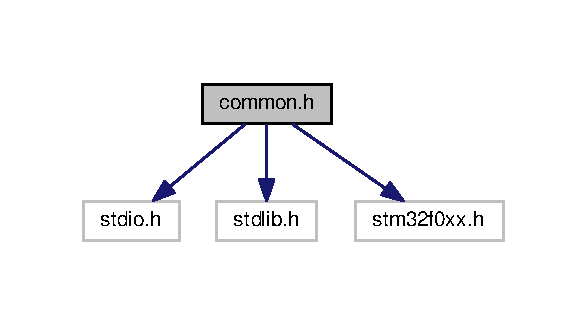
\includegraphics[width=281pt]{common_8h__incl}
\end{center}
\end{figure}
This graph shows which files directly or indirectly include this file\-:\nopagebreak
\begin{figure}[H]
\begin{center}
\leavevmode
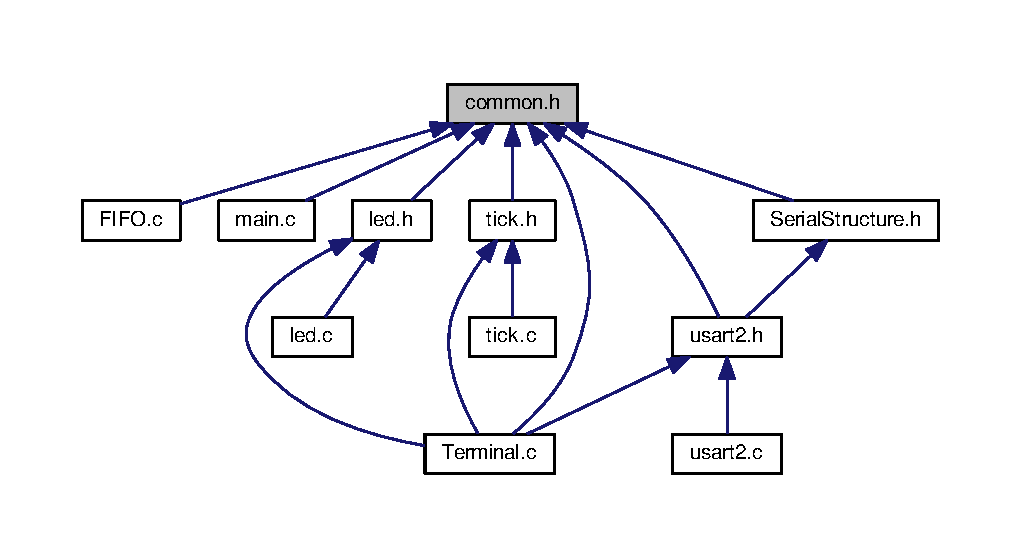
\includegraphics[width=350pt]{common_8h__dep__incl}
\end{center}
\end{figure}
\subsection*{Classes}
\begin{DoxyCompactItemize}
\item 
union \hyperlink{union_data_converter}{Data\-Converter}
\begin{DoxyCompactList}\small\item\em define the union type used to convert between types. \end{DoxyCompactList}\end{DoxyCompactItemize}
\subsection*{Macros}
\begin{DoxyCompactItemize}
\item 
\#define \hyperlink{common_8h_aa8cecfc5c5c054d2875c03e77b7be15d}{T\-R\-U\-E}~1
\begin{DoxyCompactList}\small\item\em Defines the true state. \end{DoxyCompactList}\item 
\#define \hyperlink{common_8h_aa93f0eb578d23995850d61f7d61c55c1}{F\-A\-L\-S\-E}~0
\begin{DoxyCompactList}\small\item\em Defines the false state. \end{DoxyCompactList}\item 
\#define \hyperlink{common_8h_a8fe83ac76edc595f6b98cd4a4127aed5}{E\-R\-R\-O\-R}~-\/1
\begin{DoxyCompactList}\small\item\em Defines the default error state. \end{DoxyCompactList}\item 
\#define \hyperlink{common_8h_a09b90b1d00e10094106f51f108e05dfe}{E\-R\-R\-O\-R\-\_\-\-I\-N\-V\-A\-L\-I\-D\-\_\-\-P\-O\-I\-N\-T\-E\-R}~-\/2
\begin{DoxyCompactList}\small\item\em Defines the an error for when pointer are invalid. \end{DoxyCompactList}\item 
\#define \hyperlink{common_8h_aa14dc39d52ab121ceb570f1a265385e0}{F\-I\-R\-M\-W\-A\-R\-E\-\_\-\-V\-E\-R\-S\-I\-O\-N}~\char`\"{}00.\-0001\-D\char`\"{}
\begin{DoxyCompactList}\small\item\em Firmware version D = development version of the firmware. Should only be used for testing purposes C = concession version. This version of the firmware is usual custome for a customer. see C\-O\-N\-C\-E\-S\-S\-I\-O\-N\-\_\-\-N\-U\-M\-B\-E\-R P = production version. \end{DoxyCompactList}\item 
\#define \hyperlink{common_8h_a7c770e481dd85c7ffb40e3b3edb0beb5}{H\-A\-R\-D\-W\-A\-R\-E\-\_\-\-V\-E\-R\-S\-I\-O\-N}~\char`\"{}00\char`\"{}
\begin{DoxyCompactList}\small\item\em Hardware version. \end{DoxyCompactList}\item 
\#define \hyperlink{common_8h_a4c681fec0533353b247257c82546f7cd}{C\-O\-M\-P\-I\-L\-E\-D\-\_\-\-D\-A\-T\-A\-\_\-\-T\-I\-M\-E}~\char`\"{}\mbox{[}\char`\"{} \-\_\-\-\_\-\-D\-A\-T\-E\-\_\-\-\_\- \char`\"{} \char`\"{} \-\_\-\-\_\-\-T\-I\-M\-E\-\_\-\-\_\- \char`\"{}\mbox{]}\char`\"{}
\begin{DoxyCompactList}\small\item\em Hardware version. \end{DoxyCompactList}\item 
\#define \hyperlink{common_8h_a5d95e93610ec76137962e82eebebd723}{E\-N\-\_\-\-D\-E\-B\-U\-G\-\_\-\-I\-N\-T\-E\-R\-F\-A\-C\-E}
\begin{DoxyCompactList}\small\item\em Enables the debug interface and all debug message associated. \end{DoxyCompactList}\end{DoxyCompactItemize}


\subsection{Detailed Description}
Holds all common code definitions. Author\-: Ronald Sousa () 

\subsection{Macro Definition Documentation}
\hypertarget{common_8h_a4c681fec0533353b247257c82546f7cd}{\index{common.\-h@{common.\-h}!C\-O\-M\-P\-I\-L\-E\-D\-\_\-\-D\-A\-T\-A\-\_\-\-T\-I\-M\-E@{C\-O\-M\-P\-I\-L\-E\-D\-\_\-\-D\-A\-T\-A\-\_\-\-T\-I\-M\-E}}
\index{C\-O\-M\-P\-I\-L\-E\-D\-\_\-\-D\-A\-T\-A\-\_\-\-T\-I\-M\-E@{C\-O\-M\-P\-I\-L\-E\-D\-\_\-\-D\-A\-T\-A\-\_\-\-T\-I\-M\-E}!common.h@{common.\-h}}
\subsubsection[{C\-O\-M\-P\-I\-L\-E\-D\-\_\-\-D\-A\-T\-A\-\_\-\-T\-I\-M\-E}]{\setlength{\rightskip}{0pt plus 5cm}\#define C\-O\-M\-P\-I\-L\-E\-D\-\_\-\-D\-A\-T\-A\-\_\-\-T\-I\-M\-E~\char`\"{}\mbox{[}\char`\"{} \-\_\-\-\_\-\-D\-A\-T\-E\-\_\-\-\_\- \char`\"{} \char`\"{} \-\_\-\-\_\-\-T\-I\-M\-E\-\_\-\-\_\- \char`\"{}\mbox{]}\char`\"{}}}\label{common_8h_a4c681fec0533353b247257c82546f7cd}


Hardware version. 

\hypertarget{common_8h_a5d95e93610ec76137962e82eebebd723}{\index{common.\-h@{common.\-h}!E\-N\-\_\-\-D\-E\-B\-U\-G\-\_\-\-I\-N\-T\-E\-R\-F\-A\-C\-E@{E\-N\-\_\-\-D\-E\-B\-U\-G\-\_\-\-I\-N\-T\-E\-R\-F\-A\-C\-E}}
\index{E\-N\-\_\-\-D\-E\-B\-U\-G\-\_\-\-I\-N\-T\-E\-R\-F\-A\-C\-E@{E\-N\-\_\-\-D\-E\-B\-U\-G\-\_\-\-I\-N\-T\-E\-R\-F\-A\-C\-E}!common.h@{common.\-h}}
\subsubsection[{E\-N\-\_\-\-D\-E\-B\-U\-G\-\_\-\-I\-N\-T\-E\-R\-F\-A\-C\-E}]{\setlength{\rightskip}{0pt plus 5cm}\#define E\-N\-\_\-\-D\-E\-B\-U\-G\-\_\-\-I\-N\-T\-E\-R\-F\-A\-C\-E}}\label{common_8h_a5d95e93610ec76137962e82eebebd723}


Enables the debug interface and all debug message associated. 

\hypertarget{common_8h_a8fe83ac76edc595f6b98cd4a4127aed5}{\index{common.\-h@{common.\-h}!E\-R\-R\-O\-R@{E\-R\-R\-O\-R}}
\index{E\-R\-R\-O\-R@{E\-R\-R\-O\-R}!common.h@{common.\-h}}
\subsubsection[{E\-R\-R\-O\-R}]{\setlength{\rightskip}{0pt plus 5cm}\#define E\-R\-R\-O\-R~-\/1}}\label{common_8h_a8fe83ac76edc595f6b98cd4a4127aed5}


Defines the default error state. 

\hypertarget{common_8h_a09b90b1d00e10094106f51f108e05dfe}{\index{common.\-h@{common.\-h}!E\-R\-R\-O\-R\-\_\-\-I\-N\-V\-A\-L\-I\-D\-\_\-\-P\-O\-I\-N\-T\-E\-R@{E\-R\-R\-O\-R\-\_\-\-I\-N\-V\-A\-L\-I\-D\-\_\-\-P\-O\-I\-N\-T\-E\-R}}
\index{E\-R\-R\-O\-R\-\_\-\-I\-N\-V\-A\-L\-I\-D\-\_\-\-P\-O\-I\-N\-T\-E\-R@{E\-R\-R\-O\-R\-\_\-\-I\-N\-V\-A\-L\-I\-D\-\_\-\-P\-O\-I\-N\-T\-E\-R}!common.h@{common.\-h}}
\subsubsection[{E\-R\-R\-O\-R\-\_\-\-I\-N\-V\-A\-L\-I\-D\-\_\-\-P\-O\-I\-N\-T\-E\-R}]{\setlength{\rightskip}{0pt plus 5cm}\#define E\-R\-R\-O\-R\-\_\-\-I\-N\-V\-A\-L\-I\-D\-\_\-\-P\-O\-I\-N\-T\-E\-R~-\/2}}\label{common_8h_a09b90b1d00e10094106f51f108e05dfe}


Defines the an error for when pointer are invalid. 

\hypertarget{common_8h_aa93f0eb578d23995850d61f7d61c55c1}{\index{common.\-h@{common.\-h}!F\-A\-L\-S\-E@{F\-A\-L\-S\-E}}
\index{F\-A\-L\-S\-E@{F\-A\-L\-S\-E}!common.h@{common.\-h}}
\subsubsection[{F\-A\-L\-S\-E}]{\setlength{\rightskip}{0pt plus 5cm}\#define F\-A\-L\-S\-E~0}}\label{common_8h_aa93f0eb578d23995850d61f7d61c55c1}


Defines the false state. 

\hypertarget{common_8h_aa14dc39d52ab121ceb570f1a265385e0}{\index{common.\-h@{common.\-h}!F\-I\-R\-M\-W\-A\-R\-E\-\_\-\-V\-E\-R\-S\-I\-O\-N@{F\-I\-R\-M\-W\-A\-R\-E\-\_\-\-V\-E\-R\-S\-I\-O\-N}}
\index{F\-I\-R\-M\-W\-A\-R\-E\-\_\-\-V\-E\-R\-S\-I\-O\-N@{F\-I\-R\-M\-W\-A\-R\-E\-\_\-\-V\-E\-R\-S\-I\-O\-N}!common.h@{common.\-h}}
\subsubsection[{F\-I\-R\-M\-W\-A\-R\-E\-\_\-\-V\-E\-R\-S\-I\-O\-N}]{\setlength{\rightskip}{0pt plus 5cm}\#define F\-I\-R\-M\-W\-A\-R\-E\-\_\-\-V\-E\-R\-S\-I\-O\-N~\char`\"{}00.\-0001\-D\char`\"{}}}\label{common_8h_aa14dc39d52ab121ceb570f1a265385e0}


Firmware version D = development version of the firmware. Should only be used for testing purposes C = concession version. This version of the firmware is usual custome for a customer. see C\-O\-N\-C\-E\-S\-S\-I\-O\-N\-\_\-\-N\-U\-M\-B\-E\-R P = production version. 

\begin{DoxySeeAlso}{See Also}
C\-O\-N\-C\-E\-S\-S\-I\-O\-N\-\_\-\-N\-U\-M\-B\-E\-R 
\end{DoxySeeAlso}
\hypertarget{common_8h_a7c770e481dd85c7ffb40e3b3edb0beb5}{\index{common.\-h@{common.\-h}!H\-A\-R\-D\-W\-A\-R\-E\-\_\-\-V\-E\-R\-S\-I\-O\-N@{H\-A\-R\-D\-W\-A\-R\-E\-\_\-\-V\-E\-R\-S\-I\-O\-N}}
\index{H\-A\-R\-D\-W\-A\-R\-E\-\_\-\-V\-E\-R\-S\-I\-O\-N@{H\-A\-R\-D\-W\-A\-R\-E\-\_\-\-V\-E\-R\-S\-I\-O\-N}!common.h@{common.\-h}}
\subsubsection[{H\-A\-R\-D\-W\-A\-R\-E\-\_\-\-V\-E\-R\-S\-I\-O\-N}]{\setlength{\rightskip}{0pt plus 5cm}\#define H\-A\-R\-D\-W\-A\-R\-E\-\_\-\-V\-E\-R\-S\-I\-O\-N~\char`\"{}00\char`\"{}}}\label{common_8h_a7c770e481dd85c7ffb40e3b3edb0beb5}


Hardware version. 

\hypertarget{common_8h_aa8cecfc5c5c054d2875c03e77b7be15d}{\index{common.\-h@{common.\-h}!T\-R\-U\-E@{T\-R\-U\-E}}
\index{T\-R\-U\-E@{T\-R\-U\-E}!common.h@{common.\-h}}
\subsubsection[{T\-R\-U\-E}]{\setlength{\rightskip}{0pt plus 5cm}\#define T\-R\-U\-E~1}}\label{common_8h_aa8cecfc5c5c054d2875c03e77b7be15d}


Defines the true state. 


\hypertarget{_f_i_f_o_8c}{\section{F\-I\-F\-O.\-c File Reference}
\label{_f_i_f_o_8c}\index{F\-I\-F\-O.\-c@{F\-I\-F\-O.\-c}}
}


This is our F\-I\-F\-O library.  


{\ttfamily \#include \char`\"{}common.\-h\char`\"{}}\\*
Include dependency graph for F\-I\-F\-O.\-c\-:\nopagebreak
\begin{figure}[H]
\begin{center}
\leavevmode
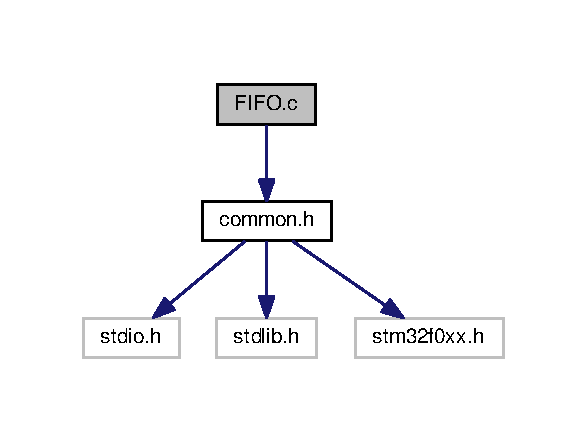
\includegraphics[width=281pt]{_f_i_f_o_8c__incl}
\end{center}
\end{figure}
\subsection*{Macros}
\begin{DoxyCompactItemize}
\item 
\hypertarget{_f_i_f_o_8c_a09cc7a19970e19234eaf82ce09b6c2ad}{\#define \hyperlink{_f_i_f_o_8c_a09cc7a19970e19234eaf82ce09b6c2ad}{F\-I\-F\-O\-\_\-\-B\-U\-F\-F\-E\-R\-\_\-\-M\-A\-X\-\_\-\-S\-I\-Z\-E}~3}\label{_f_i_f_o_8c_a09cc7a19970e19234eaf82ce09b6c2ad}

\begin{DoxyCompactList}\small\item\em defines the fifo buffer max size. \end{DoxyCompactList}\end{DoxyCompactItemize}
\subsection*{Functions}
\begin{DoxyCompactItemize}
\item 
\hypertarget{_f_i_f_o_8c_ac782a85fa346582e7b1faeb82f7cbe75}{void \hyperlink{_f_i_f_o_8c_ac782a85fa346582e7b1faeb82f7cbe75}{F\-I\-F\-O\-\_\-\-Initialiser} (void)}\label{_f_i_f_o_8c_ac782a85fa346582e7b1faeb82f7cbe75}

\begin{DoxyCompactList}\small\item\em This will init the fifo variables and clear the buffer. \end{DoxyCompactList}\item 
uint\-\_\-fast8\-\_\-t \hyperlink{_f_i_f_o_8c_a8328a1725cddf8c3b62939cb86037b9c}{F\-I\-F\-O\-\_\-\-Read} (uint8\-\_\-t $\ast$output\-Data\-Pointer)
\begin{DoxyCompactList}\small\item\em Read one bute from the buffer. Return false if we didn't. \end{DoxyCompactList}\item 
uint\-\_\-fast8\-\_\-t \hyperlink{_f_i_f_o_8c_adb6a9350a95d5de88479c528d8447521}{F\-I\-F\-O\-\_\-\-Write} (uint8\-\_\-t input\-Data)
\begin{DoxyCompactList}\small\item\em Write input\-Data into our buffer. \end{DoxyCompactList}\end{DoxyCompactItemize}


\subsection{Detailed Description}
This is our F\-I\-F\-O library. \begin{DoxyAuthor}{Author}
Ronald Sousa  
\end{DoxyAuthor}


\subsection{Function Documentation}
\hypertarget{_f_i_f_o_8c_a8328a1725cddf8c3b62939cb86037b9c}{\index{F\-I\-F\-O.\-c@{F\-I\-F\-O.\-c}!F\-I\-F\-O\-\_\-\-Read@{F\-I\-F\-O\-\_\-\-Read}}
\index{F\-I\-F\-O\-\_\-\-Read@{F\-I\-F\-O\-\_\-\-Read}!FIFO.c@{F\-I\-F\-O.\-c}}
\subsubsection[{F\-I\-F\-O\-\_\-\-Read}]{\setlength{\rightskip}{0pt plus 5cm}uint\-\_\-fast8\-\_\-t F\-I\-F\-O\-\_\-\-Read (
\begin{DoxyParamCaption}
\item[{uint8\-\_\-t $\ast$}]{output\-Data\-Pointer}
\end{DoxyParamCaption}
)}}\label{_f_i_f_o_8c_a8328a1725cddf8c3b62939cb86037b9c}


Read one bute from the buffer. Return false if we didn't. 


\begin{DoxyParams}{Parameters}
{\em output\-Data\-Pointer} & pointer to return the read value.\\
\hline
\end{DoxyParams}
\begin{DoxyReturn}{Returns}
T\-R\-U\-E = successfully read a byte rom buffer F\-A\-L\-S\-E = no data to read E\-R\-R\-O\-R = Invalid output\-Data\-Pointer pointer 
\end{DoxyReturn}
\begin{DoxyRefDesc}{Todo}
\item[\hyperlink{todo__todo000001}{Todo}]Remove me \end{DoxyRefDesc}


Here is the caller graph for this function\-:\nopagebreak
\begin{figure}[H]
\begin{center}
\leavevmode
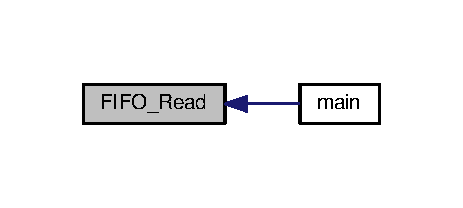
\includegraphics[width=222pt]{_f_i_f_o_8c_a8328a1725cddf8c3b62939cb86037b9c_icgraph}
\end{center}
\end{figure}


\hypertarget{_f_i_f_o_8c_adb6a9350a95d5de88479c528d8447521}{\index{F\-I\-F\-O.\-c@{F\-I\-F\-O.\-c}!F\-I\-F\-O\-\_\-\-Write@{F\-I\-F\-O\-\_\-\-Write}}
\index{F\-I\-F\-O\-\_\-\-Write@{F\-I\-F\-O\-\_\-\-Write}!FIFO.c@{F\-I\-F\-O.\-c}}
\subsubsection[{F\-I\-F\-O\-\_\-\-Write}]{\setlength{\rightskip}{0pt plus 5cm}uint\-\_\-fast8\-\_\-t F\-I\-F\-O\-\_\-\-Write (
\begin{DoxyParamCaption}
\item[{uint8\-\_\-t}]{input\-Data}
\end{DoxyParamCaption}
)}}\label{_f_i_f_o_8c_adb6a9350a95d5de88479c528d8447521}


Write input\-Data into our buffer. 


\begin{DoxyParams}{Parameters}
{\em input\-Data} & copy of the data we want to store\\
\hline
\end{DoxyParams}
\begin{DoxyReturn}{Returns}
T\-R\-U\-E = successfully writing data to our buffer F\-A\-L\-S\-E = No space in buffer 
\end{DoxyReturn}


Here is the caller graph for this function\-:\nopagebreak
\begin{figure}[H]
\begin{center}
\leavevmode
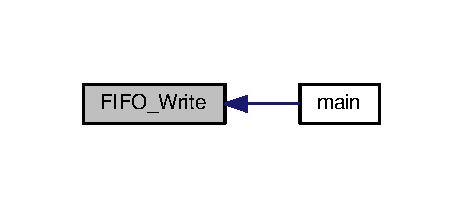
\includegraphics[width=222pt]{_f_i_f_o_8c_adb6a9350a95d5de88479c528d8447521_icgraph}
\end{center}
\end{figure}



\hypertarget{_f_i_f_o_8h}{\section{F\-I\-F\-O.\-h File Reference}
\label{_f_i_f_o_8h}\index{F\-I\-F\-O.\-h@{F\-I\-F\-O.\-h}}
}
This graph shows which files directly or indirectly include this file\-:\nopagebreak
\begin{figure}[H]
\begin{center}
\leavevmode
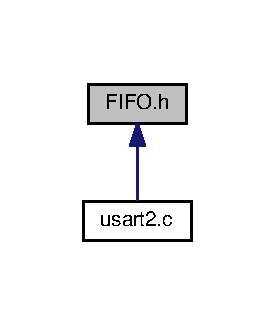
\includegraphics[width=126pt]{_f_i_f_o_8h__dep__incl}
\end{center}
\end{figure}
\subsection*{Functions}
\begin{DoxyCompactItemize}
\item 
\hypertarget{_f_i_f_o_8h_ac782a85fa346582e7b1faeb82f7cbe75}{void \hyperlink{_f_i_f_o_8h_ac782a85fa346582e7b1faeb82f7cbe75}{F\-I\-F\-O\-\_\-\-Initialiser} (void)}\label{_f_i_f_o_8h_ac782a85fa346582e7b1faeb82f7cbe75}

\begin{DoxyCompactList}\small\item\em This will init the fifo variables and clear the buffer. \end{DoxyCompactList}\item 
uint\-\_\-fast8\-\_\-t \hyperlink{_f_i_f_o_8h_adb6a9350a95d5de88479c528d8447521}{F\-I\-F\-O\-\_\-\-Write} (uint8\-\_\-t input\-Data)
\begin{DoxyCompactList}\small\item\em Write input\-Data into our buffer. \end{DoxyCompactList}\item 
uint\-\_\-fast8\-\_\-t \hyperlink{_f_i_f_o_8h_a8328a1725cddf8c3b62939cb86037b9c}{F\-I\-F\-O\-\_\-\-Read} (uint8\-\_\-t $\ast$output\-Data\-Pointer)
\begin{DoxyCompactList}\small\item\em Read one bute from the buffer. Return false if we didn't. \end{DoxyCompactList}\end{DoxyCompactItemize}


\subsection{Detailed Description}
\begin{DoxyAuthor}{Author}
Ronald Sousa  
\end{DoxyAuthor}


\subsection{Function Documentation}
\hypertarget{_f_i_f_o_8h_a8328a1725cddf8c3b62939cb86037b9c}{\index{F\-I\-F\-O.\-h@{F\-I\-F\-O.\-h}!F\-I\-F\-O\-\_\-\-Read@{F\-I\-F\-O\-\_\-\-Read}}
\index{F\-I\-F\-O\-\_\-\-Read@{F\-I\-F\-O\-\_\-\-Read}!FIFO.h@{F\-I\-F\-O.\-h}}
\subsubsection[{F\-I\-F\-O\-\_\-\-Read}]{\setlength{\rightskip}{0pt plus 5cm}uint\-\_\-fast8\-\_\-t F\-I\-F\-O\-\_\-\-Read (
\begin{DoxyParamCaption}
\item[{uint8\-\_\-t $\ast$}]{output\-Data\-Pointer}
\end{DoxyParamCaption}
)}}\label{_f_i_f_o_8h_a8328a1725cddf8c3b62939cb86037b9c}


Read one bute from the buffer. Return false if we didn't. 


\begin{DoxyParams}{Parameters}
{\em output\-Data\-Pointer} & pointer to return the read value.\\
\hline
\end{DoxyParams}
\begin{DoxyReturn}{Returns}
T\-R\-U\-E = successfully read a byte rom buffer F\-A\-L\-S\-E = no data to read E\-R\-R\-O\-R = Invalid output\-Data\-Pointer pointer 
\end{DoxyReturn}
\begin{DoxyRefDesc}{Todo}
\item[\hyperlink{todo__todo000001}{Todo}]Remove me \end{DoxyRefDesc}


Here is the caller graph for this function\-:\nopagebreak
\begin{figure}[H]
\begin{center}
\leavevmode
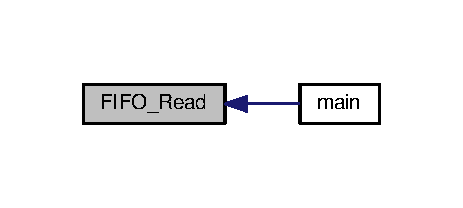
\includegraphics[width=222pt]{_f_i_f_o_8h_a8328a1725cddf8c3b62939cb86037b9c_icgraph}
\end{center}
\end{figure}


\hypertarget{_f_i_f_o_8h_adb6a9350a95d5de88479c528d8447521}{\index{F\-I\-F\-O.\-h@{F\-I\-F\-O.\-h}!F\-I\-F\-O\-\_\-\-Write@{F\-I\-F\-O\-\_\-\-Write}}
\index{F\-I\-F\-O\-\_\-\-Write@{F\-I\-F\-O\-\_\-\-Write}!FIFO.h@{F\-I\-F\-O.\-h}}
\subsubsection[{F\-I\-F\-O\-\_\-\-Write}]{\setlength{\rightskip}{0pt plus 5cm}uint\-\_\-fast8\-\_\-t F\-I\-F\-O\-\_\-\-Write (
\begin{DoxyParamCaption}
\item[{uint8\-\_\-t}]{input\-Data}
\end{DoxyParamCaption}
)}}\label{_f_i_f_o_8h_adb6a9350a95d5de88479c528d8447521}


Write input\-Data into our buffer. 


\begin{DoxyParams}{Parameters}
{\em input\-Data} & copy of the data we want to store\\
\hline
\end{DoxyParams}
\begin{DoxyReturn}{Returns}
T\-R\-U\-E = successfully writing data to our buffer F\-A\-L\-S\-E = No space in buffer 
\end{DoxyReturn}


Here is the caller graph for this function\-:\nopagebreak
\begin{figure}[H]
\begin{center}
\leavevmode
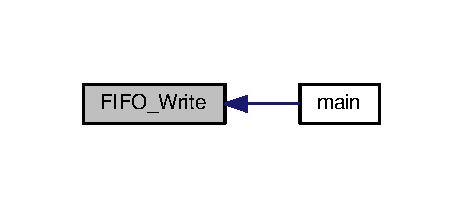
\includegraphics[width=222pt]{_f_i_f_o_8h_adb6a9350a95d5de88479c528d8447521_icgraph}
\end{center}
\end{figure}



\hypertarget{led_8c}{\section{led.\-c File Reference}
\label{led_8c}\index{led.\-c@{led.\-c}}
}


this is the L\-E\-D hardware interface layer.  


{\ttfamily \#include \char`\"{}M\-C\-U/led.\-h\char`\"{}}\\*
Include dependency graph for led.\-c\-:\nopagebreak
\begin{figure}[H]
\begin{center}
\leavevmode
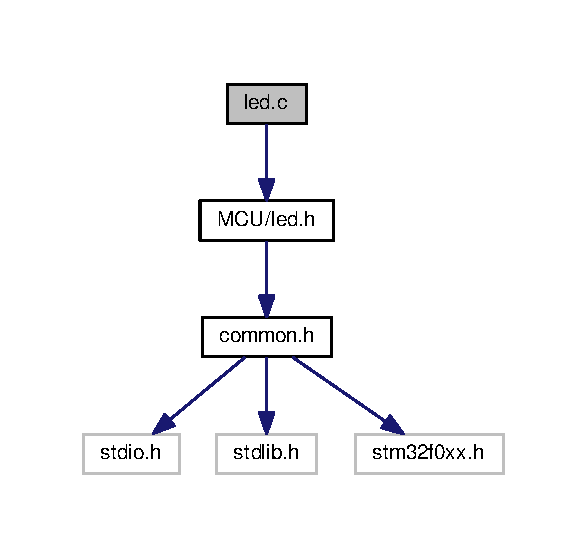
\includegraphics[width=281pt]{led_8c__incl}
\end{center}
\end{figure}
\subsection*{Macros}
\begin{DoxyCompactItemize}
\item 
\hypertarget{led_8c_ab4553be4db9860d940f81d7447173b2f}{\#define \hyperlink{led_8c_ab4553be4db9860d940f81d7447173b2f}{L\-E\-D\-\_\-\-P\-I\-N}~5}\label{led_8c_ab4553be4db9860d940f81d7447173b2f}

\begin{DoxyCompactList}\small\item\em defines the L\-E\-D pin number \end{DoxyCompactList}\end{DoxyCompactItemize}
\subsection*{Functions}
\begin{DoxyCompactItemize}
\item 
\hypertarget{led_8c_a39675df62ae72fa5af35fc7ec2e8c950}{void \hyperlink{led_8c_a39675df62ae72fa5af35fc7ec2e8c950}{Led\-\_\-\-On} (void)}\label{led_8c_a39675df62ae72fa5af35fc7ec2e8c950}

\begin{DoxyCompactList}\small\item\em Turns on the L\-E\-D. \end{DoxyCompactList}\item 
\hypertarget{led_8c_a274dbef77287444be852fe96969b3c55}{void \hyperlink{led_8c_a274dbef77287444be852fe96969b3c55}{Led\-\_\-\-Off} (void)}\label{led_8c_a274dbef77287444be852fe96969b3c55}

\begin{DoxyCompactList}\small\item\em Turns off the L\-E\-D. \end{DoxyCompactList}\item 
\hypertarget{led_8c_a5ebbd778fb3444fbfbded2130e08b33d}{void \hyperlink{led_8c_a5ebbd778fb3444fbfbded2130e08b33d}{Led\-\_\-\-Toggle} (void)}\label{led_8c_a5ebbd778fb3444fbfbded2130e08b33d}

\begin{DoxyCompactList}\small\item\em Toggle the L\-E\-D state. \end{DoxyCompactList}\item 
\hypertarget{led_8c_af1aee968a5ceeb7915921aa6d78aca23}{void \hyperlink{led_8c_af1aee968a5ceeb7915921aa6d78aca23}{Led\-\_\-\-Init} (void)}\label{led_8c_af1aee968a5ceeb7915921aa6d78aca23}

\begin{DoxyCompactList}\small\item\em Setup the L\-E\-D I\-O. \end{DoxyCompactList}\end{DoxyCompactItemize}


\subsection{Detailed Description}
this is the L\-E\-D hardware interface layer. Author\-: Ronald Sousa () 
\hypertarget{led_8h}{\section{led.\-h File Reference}
\label{led_8h}\index{led.\-h@{led.\-h}}
}
{\ttfamily \#include \char`\"{}common.\-h\char`\"{}}\\*
Include dependency graph for led.\-h\-:\nopagebreak
\begin{figure}[H]
\begin{center}
\leavevmode
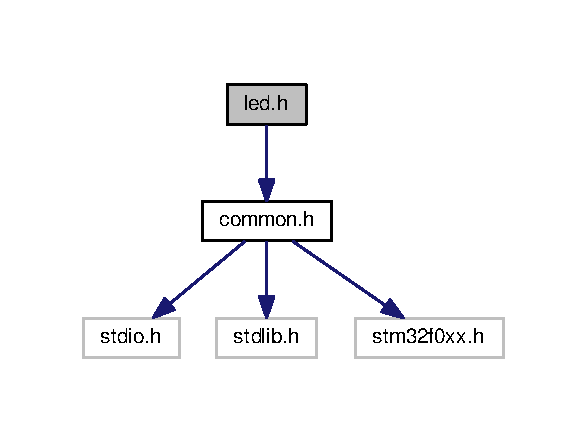
\includegraphics[width=281pt]{led_8h__incl}
\end{center}
\end{figure}
This graph shows which files directly or indirectly include this file\-:\nopagebreak
\begin{figure}[H]
\begin{center}
\leavevmode
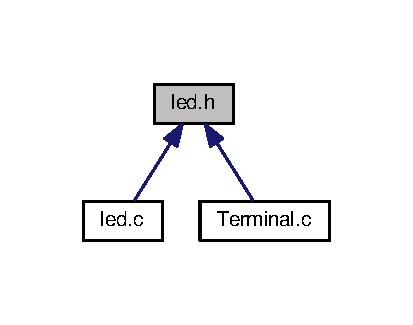
\includegraphics[width=182pt]{led_8h__dep__incl}
\end{center}
\end{figure}
\subsection*{Functions}
\begin{DoxyCompactItemize}
\item 
\hypertarget{led_8h_af1aee968a5ceeb7915921aa6d78aca23}{void \hyperlink{led_8h_af1aee968a5ceeb7915921aa6d78aca23}{Led\-\_\-\-Init} (void)}\label{led_8h_af1aee968a5ceeb7915921aa6d78aca23}

\begin{DoxyCompactList}\small\item\em Setup the L\-E\-D I\-O. \end{DoxyCompactList}\item 
\hypertarget{led_8h_a39675df62ae72fa5af35fc7ec2e8c950}{void \hyperlink{led_8h_a39675df62ae72fa5af35fc7ec2e8c950}{Led\-\_\-\-On} (void)}\label{led_8h_a39675df62ae72fa5af35fc7ec2e8c950}

\begin{DoxyCompactList}\small\item\em Turns on the L\-E\-D. \end{DoxyCompactList}\item 
\hypertarget{led_8h_a274dbef77287444be852fe96969b3c55}{void \hyperlink{led_8h_a274dbef77287444be852fe96969b3c55}{Led\-\_\-\-Off} (void)}\label{led_8h_a274dbef77287444be852fe96969b3c55}

\begin{DoxyCompactList}\small\item\em Turns off the L\-E\-D. \end{DoxyCompactList}\item 
\hypertarget{led_8h_a5ebbd778fb3444fbfbded2130e08b33d}{void \hyperlink{led_8h_a5ebbd778fb3444fbfbded2130e08b33d}{Led\-\_\-\-Toggle} (void)}\label{led_8h_a5ebbd778fb3444fbfbded2130e08b33d}

\begin{DoxyCompactList}\small\item\em Toggle the L\-E\-D state. \end{DoxyCompactList}\end{DoxyCompactItemize}


\subsection{Detailed Description}
Author\-: Ronald Sousa () 
\hypertarget{main_8c}{\section{main.\-c File Reference}
\label{main_8c}\index{main.\-c@{main.\-c}}
}


This is the main program code.  


{\ttfamily \#include \char`\"{}common.\-h\char`\"{}}\\*
{\ttfamily \#include \char`\"{}M\-C\-U/led.\-h\char`\"{}}\\*
{\ttfamily \#include \char`\"{}M\-C\-U/usart2.\-h\char`\"{}}\\*
{\ttfamily \#include \char`\"{}M\-C\-U/tick.\-h\char`\"{}}\\*
{\ttfamily \#include \char`\"{}F\-I\-F\-O.\-h\char`\"{}}\\*
Include dependency graph for main.\-c\-:\nopagebreak
\begin{figure}[H]
\begin{center}
\leavevmode
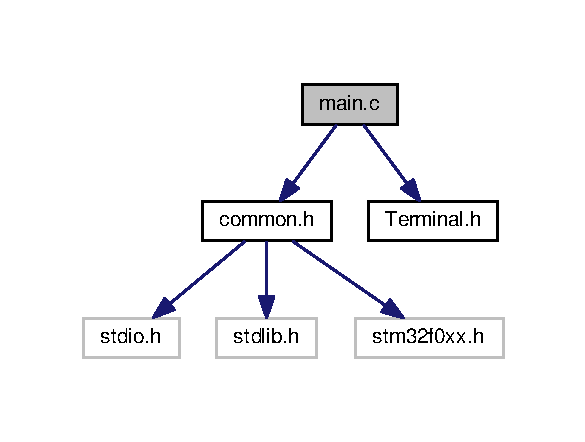
\includegraphics[width=350pt]{main_8c__incl}
\end{center}
\end{figure}
\subsection*{Functions}
\begin{DoxyCompactItemize}
\item 
\hypertarget{main_8c_a6288eba0f8e8ad3ab1544ad731eb7667}{void \hyperlink{main_8c_a6288eba0f8e8ad3ab1544ad731eb7667}{main} (void)}\label{main_8c_a6288eba0f8e8ad3ab1544ad731eb7667}

\begin{DoxyCompactList}\small\item\em the first user code function to be called after the A\-R\-M M0 has initial. \end{DoxyCompactList}\end{DoxyCompactItemize}


\subsection{Detailed Description}
This is the main program code. \begin{DoxyAuthor}{Author}
Ronald Sousa (Opticalworm) 
\end{DoxyAuthor}

\hypertarget{_serial_structure_8h}{\section{Serial\-Structure.\-h File Reference}
\label{_serial_structure_8h}\index{Serial\-Structure.\-h@{Serial\-Structure.\-h}}
}


define the serial interface layer structure  


{\ttfamily \#include \char`\"{}../common.\-h\char`\"{}}\\*
Include dependency graph for Serial\-Structure.\-h\-:\nopagebreak
\begin{figure}[H]
\begin{center}
\leavevmode
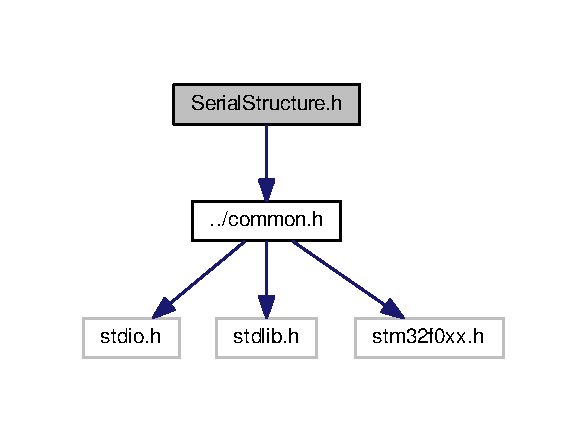
\includegraphics[width=281pt]{_serial_structure_8h__incl}
\end{center}
\end{figure}
This graph shows which files directly or indirectly include this file\-:\nopagebreak
\begin{figure}[H]
\begin{center}
\leavevmode
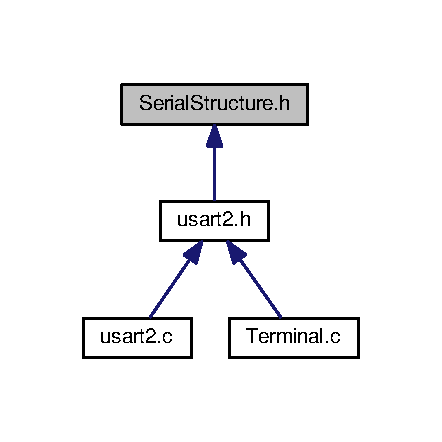
\includegraphics[width=196pt]{_serial_structure_8h__dep__incl}
\end{center}
\end{figure}
\subsection*{Classes}
\begin{DoxyCompactItemize}
\item 
struct \hyperlink{struct_serial_interface}{Serial\-Interface}
\begin{DoxyCompactList}\small\item\em define the standard serial interface \end{DoxyCompactList}\end{DoxyCompactItemize}


\subsection{Detailed Description}
define the serial interface layer structure \begin{DoxyAuthor}{Author}
Ronald Sousa  www.\-Hash\-Define\-Electronics.\-com  Hash Define Electronics Ltd 
\end{DoxyAuthor}

\hypertarget{stm32f0xx__conf_8h}{\section{stm32f0xx\-\_\-conf.\-h File Reference}
\label{stm32f0xx__conf_8h}\index{stm32f0xx\-\_\-conf.\-h@{stm32f0xx\-\_\-conf.\-h}}
}
{\ttfamily \#include \char`\"{}stm32f0xx\-\_\-adc.\-h\char`\"{}}\\*
{\ttfamily \#include \char`\"{}stm32f0xx\-\_\-can.\-h\char`\"{}}\\*
{\ttfamily \#include \char`\"{}stm32f0xx\-\_\-cec.\-h\char`\"{}}\\*
{\ttfamily \#include \char`\"{}stm32f0xx\-\_\-crc.\-h\char`\"{}}\\*
{\ttfamily \#include \char`\"{}stm32f0xx\-\_\-crs.\-h\char`\"{}}\\*
{\ttfamily \#include \char`\"{}stm32f0xx\-\_\-comp.\-h\char`\"{}}\\*
{\ttfamily \#include \char`\"{}stm32f0xx\-\_\-dac.\-h\char`\"{}}\\*
{\ttfamily \#include \char`\"{}stm32f0xx\-\_\-dbgmcu.\-h\char`\"{}}\\*
{\ttfamily \#include \char`\"{}stm32f0xx\-\_\-dma.\-h\char`\"{}}\\*
{\ttfamily \#include \char`\"{}stm32f0xx\-\_\-exti.\-h\char`\"{}}\\*
{\ttfamily \#include \char`\"{}stm32f0xx\-\_\-flash.\-h\char`\"{}}\\*
{\ttfamily \#include \char`\"{}stm32f0xx\-\_\-gpio.\-h\char`\"{}}\\*
{\ttfamily \#include \char`\"{}stm32f0xx\-\_\-syscfg.\-h\char`\"{}}\\*
{\ttfamily \#include \char`\"{}stm32f0xx\-\_\-i2c.\-h\char`\"{}}\\*
{\ttfamily \#include \char`\"{}stm32f0xx\-\_\-iwdg.\-h\char`\"{}}\\*
{\ttfamily \#include \char`\"{}stm32f0xx\-\_\-pwr.\-h\char`\"{}}\\*
{\ttfamily \#include \char`\"{}stm32f0xx\-\_\-rcc.\-h\char`\"{}}\\*
{\ttfamily \#include \char`\"{}stm32f0xx\-\_\-rtc.\-h\char`\"{}}\\*
{\ttfamily \#include \char`\"{}stm32f0xx\-\_\-spi.\-h\char`\"{}}\\*
{\ttfamily \#include \char`\"{}stm32f0xx\-\_\-tim.\-h\char`\"{}}\\*
{\ttfamily \#include \char`\"{}stm32f0xx\-\_\-usart.\-h\char`\"{}}\\*
{\ttfamily \#include \char`\"{}stm32f0xx\-\_\-wwdg.\-h\char`\"{}}\\*
{\ttfamily \#include \char`\"{}stm32f0xx\-\_\-misc.\-h\char`\"{}}\\*
Include dependency graph for stm32f0xx\-\_\-conf.\-h\-:
\nopagebreak
\begin{figure}[H]
\begin{center}
\leavevmode
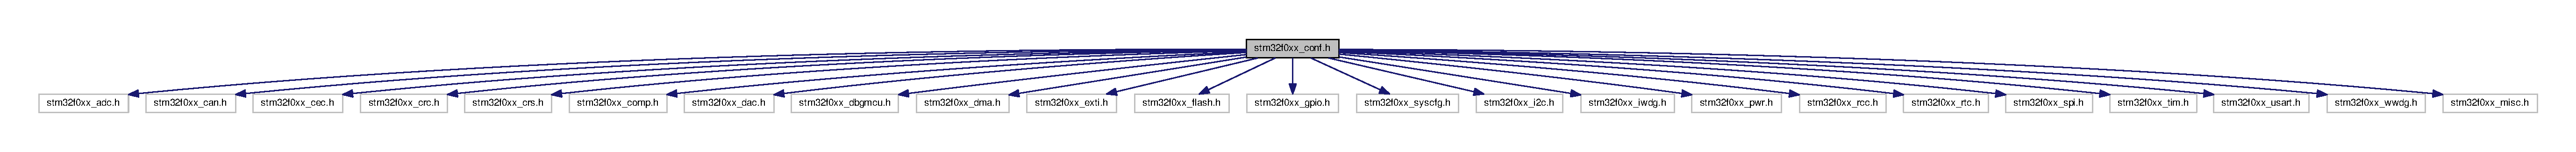
\includegraphics[width=350pt]{stm32f0xx__conf_8h__incl}
\end{center}
\end{figure}
\subsection*{Macros}
\begin{DoxyCompactItemize}
\item 
\#define \hyperlink{stm32f0xx__conf_8h_a631dea7b230e600555f979c62af1de21}{assert\-\_\-param}(expr)~((void)0)
\end{DoxyCompactItemize}


\subsection{Macro Definition Documentation}
\hypertarget{stm32f0xx__conf_8h_a631dea7b230e600555f979c62af1de21}{\index{stm32f0xx\-\_\-conf.\-h@{stm32f0xx\-\_\-conf.\-h}!assert\-\_\-param@{assert\-\_\-param}}
\index{assert\-\_\-param@{assert\-\_\-param}!stm32f0xx_conf.h@{stm32f0xx\-\_\-conf.\-h}}
\subsubsection[{assert\-\_\-param}]{\setlength{\rightskip}{0pt plus 5cm}\#define assert\-\_\-param(
\begin{DoxyParamCaption}
\item[{}]{expr}
\end{DoxyParamCaption}
)~((void)0)}}\label{stm32f0xx__conf_8h_a631dea7b230e600555f979c62af1de21}

\hypertarget{_terminal_8c}{\section{Terminal.\-c File Reference}
\label{_terminal_8c}\index{Terminal.\-c@{Terminal.\-c}}
}
{\ttfamily \#include \char`\"{}common.\-h\char`\"{}}\\*
{\ttfamily \#include \char`\"{}M\-C\-U/led.\-h\char`\"{}}\\*
{\ttfamily \#include \char`\"{}M\-C\-U/usart2.\-h\char`\"{}}\\*
{\ttfamily \#include \char`\"{}M\-C\-U/tick.\-h\char`\"{}}\\*
Include dependency graph for Terminal.\-c\-:\nopagebreak
\begin{figure}[H]
\begin{center}
\leavevmode
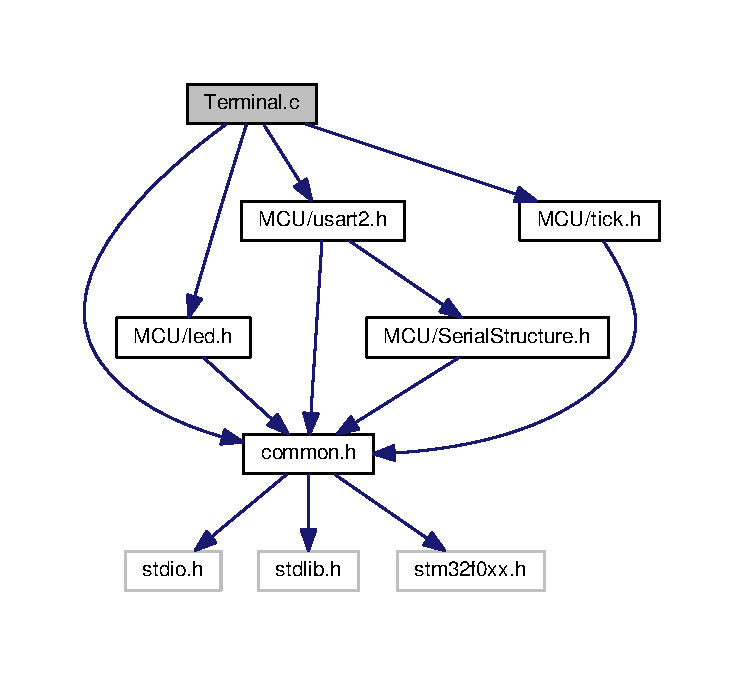
\includegraphics[width=350pt]{_terminal_8c__incl}
\end{center}
\end{figure}
\subsection*{Classes}
\begin{DoxyCompactItemize}
\item 
struct \hyperlink{struct_param_structure_type}{Param\-Structure\-Type}
\begin{DoxyCompactList}\small\item\em Defines the parameter data type. \end{DoxyCompactList}\item 
struct \hyperlink{struct_list_of_parameter_structure_type}{List\-Of\-Parameter\-Structure\-Type}
\begin{DoxyCompactList}\small\item\em Defines the list of parameter data structure. \end{DoxyCompactList}\end{DoxyCompactItemize}
\subsection*{Macros}
\begin{DoxyCompactItemize}
\item 
\#define \hyperlink{_terminal_8c_a4254377693b37d0990025e2a86a1ec0d}{T\-E\-R\-M\-I\-N\-A\-L\-\_\-\-B\-U\-F\-F\-E\-R\-\_\-\-S\-I\-Z\-E}~25
\begin{DoxyCompactList}\small\item\em Defines our terminal buffer size which in turn set the longest command. \end{DoxyCompactList}\end{DoxyCompactItemize}
\subsection*{Functions}
\begin{DoxyCompactItemize}
\item 
void \hyperlink{_terminal_8c_acc9b80fa13f248f795d961b1817b7d4b}{Terminal\-\_\-\-Init} (void)
\begin{DoxyCompactList}\small\item\em Init the terminal program. \end{DoxyCompactList}\item 
int\-\_\-fast8\-\_\-t \hyperlink{_terminal_8c_a683f74bf787b52b7f357e405c6c2819c}{Terminal\-\_\-\-Process} (void)
\begin{DoxyCompactList}\small\item\em process the buffer data and extract the commands \end{DoxyCompactList}\end{DoxyCompactItemize}


\subsection{Detailed Description}
\begin{DoxyAuthor}{Author}
Ronald Sousa  
\end{DoxyAuthor}


\subsection{Macro Definition Documentation}
\hypertarget{_terminal_8c_a4254377693b37d0990025e2a86a1ec0d}{\index{Terminal.\-c@{Terminal.\-c}!T\-E\-R\-M\-I\-N\-A\-L\-\_\-\-B\-U\-F\-F\-E\-R\-\_\-\-S\-I\-Z\-E@{T\-E\-R\-M\-I\-N\-A\-L\-\_\-\-B\-U\-F\-F\-E\-R\-\_\-\-S\-I\-Z\-E}}
\index{T\-E\-R\-M\-I\-N\-A\-L\-\_\-\-B\-U\-F\-F\-E\-R\-\_\-\-S\-I\-Z\-E@{T\-E\-R\-M\-I\-N\-A\-L\-\_\-\-B\-U\-F\-F\-E\-R\-\_\-\-S\-I\-Z\-E}!Terminal.c@{Terminal.\-c}}
\subsubsection[{T\-E\-R\-M\-I\-N\-A\-L\-\_\-\-B\-U\-F\-F\-E\-R\-\_\-\-S\-I\-Z\-E}]{\setlength{\rightskip}{0pt plus 5cm}\#define T\-E\-R\-M\-I\-N\-A\-L\-\_\-\-B\-U\-F\-F\-E\-R\-\_\-\-S\-I\-Z\-E~25}}\label{_terminal_8c_a4254377693b37d0990025e2a86a1ec0d}


Defines our terminal buffer size which in turn set the longest command. 



\subsection{Function Documentation}
\hypertarget{_terminal_8c_acc9b80fa13f248f795d961b1817b7d4b}{\index{Terminal.\-c@{Terminal.\-c}!Terminal\-\_\-\-Init@{Terminal\-\_\-\-Init}}
\index{Terminal\-\_\-\-Init@{Terminal\-\_\-\-Init}!Terminal.c@{Terminal.\-c}}
\subsubsection[{Terminal\-\_\-\-Init}]{\setlength{\rightskip}{0pt plus 5cm}void Terminal\-\_\-\-Init (
\begin{DoxyParamCaption}
\item[{void}]{}
\end{DoxyParamCaption}
)}}\label{_terminal_8c_acc9b80fa13f248f795d961b1817b7d4b}


Init the terminal program. 



Here is the call graph for this function\-:
\nopagebreak
\begin{figure}[H]
\begin{center}
\leavevmode
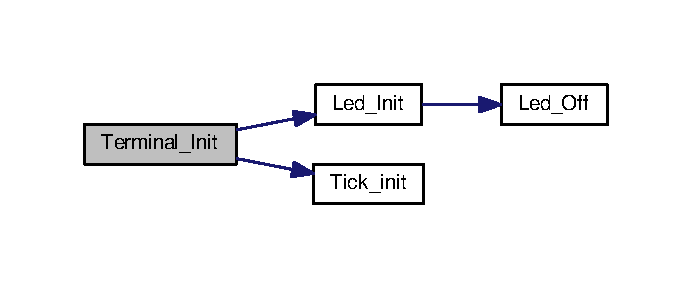
\includegraphics[width=332pt]{_terminal_8c_acc9b80fa13f248f795d961b1817b7d4b_cgraph}
\end{center}
\end{figure}




Here is the caller graph for this function\-:
\nopagebreak
\begin{figure}[H]
\begin{center}
\leavevmode
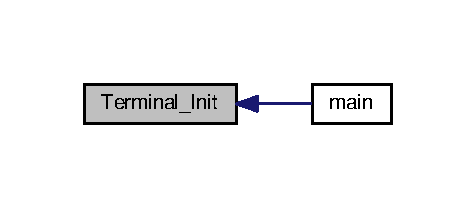
\includegraphics[width=228pt]{_terminal_8c_acc9b80fa13f248f795d961b1817b7d4b_icgraph}
\end{center}
\end{figure}


\hypertarget{_terminal_8c_a683f74bf787b52b7f357e405c6c2819c}{\index{Terminal.\-c@{Terminal.\-c}!Terminal\-\_\-\-Process@{Terminal\-\_\-\-Process}}
\index{Terminal\-\_\-\-Process@{Terminal\-\_\-\-Process}!Terminal.c@{Terminal.\-c}}
\subsubsection[{Terminal\-\_\-\-Process}]{\setlength{\rightskip}{0pt plus 5cm}int\-\_\-fast8\-\_\-t Terminal\-\_\-\-Process (
\begin{DoxyParamCaption}
\item[{void}]{}
\end{DoxyParamCaption}
)}}\label{_terminal_8c_a683f74bf787b52b7f357e405c6c2819c}


process the buffer data and extract the commands 

\begin{DoxyReturn}{Returns}
T\-R\-U\-E success. F\-A\-L\-S\-E no error
\end{DoxyReturn}
\begin{DoxyRefDesc}{Todo}
\item[\hyperlink{todo__todo000005}{Todo}]update the document return state value. need to implement \end{DoxyRefDesc}
\begin{DoxyRefDesc}{Todo}
\item[\hyperlink{todo__todo000006}{Todo}]call the process data \end{DoxyRefDesc}


Here is the caller graph for this function\-:\nopagebreak
\begin{figure}[H]
\begin{center}
\leavevmode
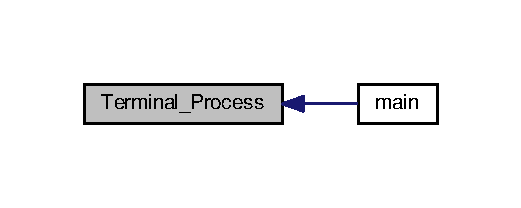
\includegraphics[width=250pt]{_terminal_8c_a683f74bf787b52b7f357e405c6c2819c_icgraph}
\end{center}
\end{figure}



\hypertarget{_terminal_8h}{\section{Terminal.\-h File Reference}
\label{_terminal_8h}\index{Terminal.\-h@{Terminal.\-h}}
}
This graph shows which files directly or indirectly include this file\-:\nopagebreak
\begin{figure}[H]
\begin{center}
\leavevmode
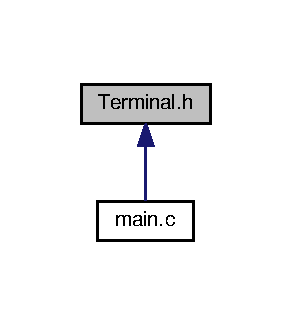
\includegraphics[width=140pt]{_terminal_8h__dep__incl}
\end{center}
\end{figure}
\subsection*{Functions}
\begin{DoxyCompactItemize}
\item 
void \hyperlink{_terminal_8h_acc9b80fa13f248f795d961b1817b7d4b}{Terminal\-\_\-\-Init} (void)
\begin{DoxyCompactList}\small\item\em Init the terminal program. \end{DoxyCompactList}\item 
uint\-\_\-fast8\-\_\-t \hyperlink{_terminal_8h_a8939cfce56b8f95a2a322c973190204e}{Terminal\-\_\-\-Process} (void)
\begin{DoxyCompactList}\small\item\em process the buffer data and extract the commands \end{DoxyCompactList}\end{DoxyCompactItemize}


\subsection{Detailed Description}
\begin{DoxyAuthor}{Author}
Ronald Sousa  
\end{DoxyAuthor}


\subsection{Function Documentation}
\hypertarget{_terminal_8h_acc9b80fa13f248f795d961b1817b7d4b}{\index{Terminal.\-h@{Terminal.\-h}!Terminal\-\_\-\-Init@{Terminal\-\_\-\-Init}}
\index{Terminal\-\_\-\-Init@{Terminal\-\_\-\-Init}!Terminal.h@{Terminal.\-h}}
\subsubsection[{Terminal\-\_\-\-Init}]{\setlength{\rightskip}{0pt plus 5cm}void Terminal\-\_\-\-Init (
\begin{DoxyParamCaption}
\item[{void}]{}
\end{DoxyParamCaption}
)}}\label{_terminal_8h_acc9b80fa13f248f795d961b1817b7d4b}


Init the terminal program. 



Here is the call graph for this function\-:
\nopagebreak
\begin{figure}[H]
\begin{center}
\leavevmode
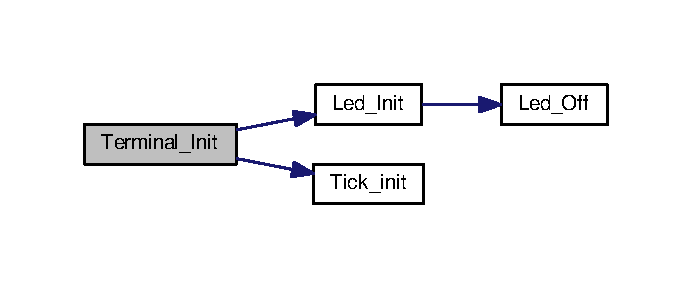
\includegraphics[width=332pt]{_terminal_8h_acc9b80fa13f248f795d961b1817b7d4b_cgraph}
\end{center}
\end{figure}




Here is the caller graph for this function\-:
\nopagebreak
\begin{figure}[H]
\begin{center}
\leavevmode
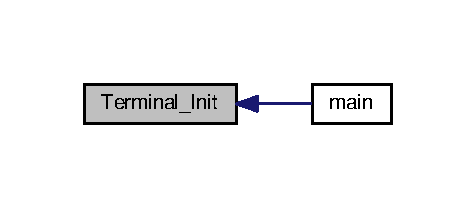
\includegraphics[width=228pt]{_terminal_8h_acc9b80fa13f248f795d961b1817b7d4b_icgraph}
\end{center}
\end{figure}


\hypertarget{_terminal_8h_a8939cfce56b8f95a2a322c973190204e}{\index{Terminal.\-h@{Terminal.\-h}!Terminal\-\_\-\-Process@{Terminal\-\_\-\-Process}}
\index{Terminal\-\_\-\-Process@{Terminal\-\_\-\-Process}!Terminal.h@{Terminal.\-h}}
\subsubsection[{Terminal\-\_\-\-Process}]{\setlength{\rightskip}{0pt plus 5cm}uint\-\_\-fast8\-\_\-t Terminal\-\_\-\-Process (
\begin{DoxyParamCaption}
\item[{void}]{}
\end{DoxyParamCaption}
)}}\label{_terminal_8h_a8939cfce56b8f95a2a322c973190204e}


process the buffer data and extract the commands 

\begin{DoxyReturn}{Returns}
T\-R\-U\-E success. F\-A\-L\-S\-E no error
\end{DoxyReturn}
\begin{DoxyRefDesc}{Todo}
\item[\hyperlink{todo__todo000005}{Todo}]update the document return state value. need to implement \end{DoxyRefDesc}
\begin{DoxyRefDesc}{Todo}
\item[\hyperlink{todo__todo000006}{Todo}]call the process data \end{DoxyRefDesc}


Here is the caller graph for this function\-:\nopagebreak
\begin{figure}[H]
\begin{center}
\leavevmode
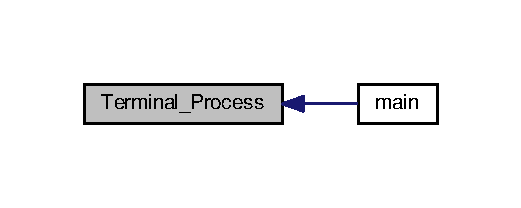
\includegraphics[width=250pt]{_terminal_8h_a8939cfce56b8f95a2a322c973190204e_icgraph}
\end{center}
\end{figure}



\hypertarget{tick_8c}{\section{tick.\-c File Reference}
\label{tick_8c}\index{tick.\-c@{tick.\-c}}
}


implements mili-\/second tick counter.  


{\ttfamily \#include \char`\"{}M\-C\-U/tick.\-h\char`\"{}}\\*
Include dependency graph for tick.\-c\-:\nopagebreak
\begin{figure}[H]
\begin{center}
\leavevmode
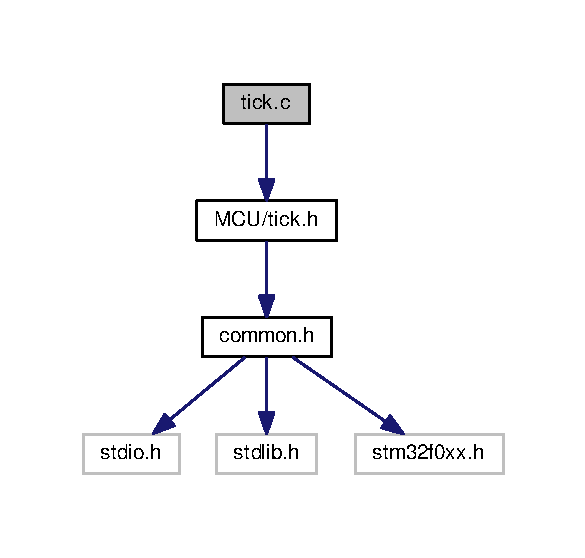
\includegraphics[width=281pt]{tick_8c__incl}
\end{center}
\end{figure}
\subsection*{Macros}
\begin{DoxyCompactItemize}
\item 
\hypertarget{tick_8c_a290a7b04bb56e02e733a35599442a915}{\#define \hyperlink{tick_8c_a290a7b04bb56e02e733a35599442a915}{T\-I\-M\-E\-R\-\_\-\-F\-R\-E\-Q\-U\-E\-N\-C\-Y\-\_\-\-H\-Z}~1000}\label{tick_8c_a290a7b04bb56e02e733a35599442a915}

\begin{DoxyCompactList}\small\item\em defines the frequency we want the system tick to trigger. for 1ms = 1/1000hz \end{DoxyCompactList}\end{DoxyCompactItemize}
\subsection*{Functions}
\begin{DoxyCompactItemize}
\item 
\hypertarget{tick_8c_ade660961e7af4755750dd6ff81535e68}{void \hyperlink{tick_8c_ade660961e7af4755750dd6ff81535e68}{Tick\-\_\-init} (void)}\label{tick_8c_ade660961e7af4755750dd6ff81535e68}

\begin{DoxyCompactList}\small\item\em setup the A\-R\-M M0 tick counter to trigger every 1ms \end{DoxyCompactList}\item 
uint32\-\_\-t \hyperlink{tick_8c_a5018c28a90fe9864e870a712c8e2b571}{Tick\-\_\-\-Get\-Ms} (void)
\begin{DoxyCompactList}\small\item\em return the number of mili-\/seconds since power up. \end{DoxyCompactList}\item 
void \hyperlink{tick_8c_a01864fcfa99d364250b9e3e10390ff93}{Tick\-\_\-\-Delay\-Ms} (uint32\-\_\-t delay\-Ms)
\begin{DoxyCompactList}\small\item\em this is a blocking delay. \end{DoxyCompactList}\item 
int\-\_\-fast8\-\_\-t \hyperlink{tick_8c_a700a086c5fb6a2a2491026af0fda77a8}{Tick\-\_\-\-Delay\-Ms\-\_\-\-Non\-Blocking} (uint\-\_\-fast8\-\_\-t reset, \hyperlink{struct_tick_type}{Tick\-Type} $\ast$config)
\begin{DoxyCompactList}\small\item\em Non-\/blocking delay in ms. \end{DoxyCompactList}\item 
void \hyperlink{tick_8c_ab5e09814056d617c521549e542639b7e}{Sys\-Tick\-\_\-\-Handler} (void)
\begin{DoxyCompactList}\small\item\em A\-R\-M M0 hardware interrupt. This should trigger every 1 ms and update Tick\-Counter. \end{DoxyCompactList}\end{DoxyCompactItemize}


\subsection{Detailed Description}
implements mili-\/second tick counter. Author\-: Ronald Sousa (Opticalworm) 

\subsection{Function Documentation}
\hypertarget{tick_8c_ab5e09814056d617c521549e542639b7e}{\index{tick.\-c@{tick.\-c}!Sys\-Tick\-\_\-\-Handler@{Sys\-Tick\-\_\-\-Handler}}
\index{Sys\-Tick\-\_\-\-Handler@{Sys\-Tick\-\_\-\-Handler}!tick.c@{tick.\-c}}
\subsubsection[{Sys\-Tick\-\_\-\-Handler}]{\setlength{\rightskip}{0pt plus 5cm}void Sys\-Tick\-\_\-\-Handler (
\begin{DoxyParamCaption}
\item[{void}]{}
\end{DoxyParamCaption}
)}}\label{tick_8c_ab5e09814056d617c521549e542639b7e}


A\-R\-M M0 hardware interrupt. This should trigger every 1 ms and update Tick\-Counter. 

\begin{DoxySeeAlso}{See Also}
Tick\-Counter 
\end{DoxySeeAlso}
\hypertarget{tick_8c_a01864fcfa99d364250b9e3e10390ff93}{\index{tick.\-c@{tick.\-c}!Tick\-\_\-\-Delay\-Ms@{Tick\-\_\-\-Delay\-Ms}}
\index{Tick\-\_\-\-Delay\-Ms@{Tick\-\_\-\-Delay\-Ms}!tick.c@{tick.\-c}}
\subsubsection[{Tick\-\_\-\-Delay\-Ms}]{\setlength{\rightskip}{0pt plus 5cm}void Tick\-\_\-\-Delay\-Ms (
\begin{DoxyParamCaption}
\item[{uint32\-\_\-t}]{delay\-Ms}
\end{DoxyParamCaption}
)}}\label{tick_8c_a01864fcfa99d364250b9e3e10390ff93}


this is a blocking delay. 


\begin{DoxyCode}
\textcolor{preprocessor}{ #include "\hyperlink{common_8h}{common.h}"}
\textcolor{preprocessor}{ #include "\hyperlink{led_8h}{MCU/led.h}"}
\textcolor{preprocessor}{ #include "\hyperlink{tick_8h}{MCU/tick.h}"}

 \textcolor{keywordtype}{void} \hyperlink{main_8c_a6288eba0f8e8ad3ab1544ad731eb7667}{main}(\textcolor{keywordtype}{void}) \{

     \hyperlink{led_8c_af1aee968a5ceeb7915921aa6d78aca23}{Led\_Init}();
     \hyperlink{tick_8c_ade660961e7af4755750dd6ff81535e68}{Tick\_init}();

     \textcolor{keywordflow}{for}( ;;) \{
       \hyperlink{tick_8c_a01864fcfa99d364250b9e3e10390ff93}{Tick\_DelayMs}(1000); \textcolor{comment}{// delay 1s;}
       \hyperlink{led_8c_a5ebbd778fb3444fbfbded2130e08b33d}{Led\_Toggle}();
     \}
\}
\end{DoxyCode}



\begin{DoxyParams}{Parameters}
{\em delay\-Ms} & how long to delay for. \\
\hline
\end{DoxyParams}
\hypertarget{tick_8c_a700a086c5fb6a2a2491026af0fda77a8}{\index{tick.\-c@{tick.\-c}!Tick\-\_\-\-Delay\-Ms\-\_\-\-Non\-Blocking@{Tick\-\_\-\-Delay\-Ms\-\_\-\-Non\-Blocking}}
\index{Tick\-\_\-\-Delay\-Ms\-\_\-\-Non\-Blocking@{Tick\-\_\-\-Delay\-Ms\-\_\-\-Non\-Blocking}!tick.c@{tick.\-c}}
\subsubsection[{Tick\-\_\-\-Delay\-Ms\-\_\-\-Non\-Blocking}]{\setlength{\rightskip}{0pt plus 5cm}int\-\_\-fast8\-\_\-t Tick\-\_\-\-Delay\-Ms\-\_\-\-Non\-Blocking (
\begin{DoxyParamCaption}
\item[{uint\-\_\-fast8\-\_\-t}]{reset, }
\item[{{\bf Tick\-Type} $\ast$}]{config}
\end{DoxyParamCaption}
)}}\label{tick_8c_a700a086c5fb6a2a2491026af0fda77a8}


Non-\/blocking delay in ms. 


\begin{DoxyCode}
\textcolor{preprocessor}{ #include "\hyperlink{common_8h}{common.h}"}
\textcolor{preprocessor}{ #include "\hyperlink{led_8h}{MCU/led.h}"}
\textcolor{preprocessor}{ #include "\hyperlink{tick_8h}{MCU/tick.h}"}

 \textcolor{keywordtype}{void} \hyperlink{main_8c_a6288eba0f8e8ad3ab1544ad731eb7667}{main}(\textcolor{keywordtype}{void}) \{
     \hyperlink{struct_tick_type}{TickType} Delay;
     Delay.\hyperlink{struct_tick_type_ae24ecd63a2b008c5c9a6864cbb3b30a7}{DelayMs} = 1000; \textcolor{comment}{//set to 1s}

     \hyperlink{led_8c_af1aee968a5ceeb7915921aa6d78aca23}{Led\_Init}();
     \hyperlink{tick_8c_ade660961e7af4755750dd6ff81535e68}{Tick\_init}();

     \textcolor{comment}{// reset the counter}
     \hyperlink{tick_8c_a700a086c5fb6a2a2491026af0fda77a8}{Tick\_DelayMs\_NonBlocking}(\hyperlink{common_8h_aa8cecfc5c5c054d2875c03e77b7be15d}{TRUE}, &Delay);

     \textcolor{keywordflow}{for}( ;;) \{

         \textcolor{keywordflow}{if}(\hyperlink{tick_8c_a700a086c5fb6a2a2491026af0fda77a8}{Tick\_DelayMs\_NonBlocking}(\hyperlink{common_8h_aa8cecfc5c5c054d2875c03e77b7be15d}{TRUE}, &Delay)) \{
             \textcolor{comment}{// Delay has been reached}

             \hyperlink{tick_8c_a700a086c5fb6a2a2491026af0fda77a8}{Tick\_DelayMs\_NonBlocking}(\hyperlink{common_8h_aa8cecfc5c5c054d2875c03e77b7be15d}{TRUE}, &Delay);
             \hyperlink{led_8c_a5ebbd778fb3444fbfbded2130e08b33d}{Led\_Toggle}();
             \}
         \textcolor{keywordflow}{else} \{
             \textcolor{comment}{// User code when the code delay hasn't passed}
             \}

     \}
\}
\end{DoxyCode}



\begin{DoxyParams}{Parameters}
{\em reset} & true = reset timer start value/ false = Check if time has lapsed \\
\hline
{\em config} & delay setting\\
\hline
\end{DoxyParams}
\begin{DoxyReturn}{Returns}
1 = the desire delay has been reached. 0 = not reached the desire delay time. -\/1 = config point is null 
\end{DoxyReturn}


Here is the call graph for this function\-:\nopagebreak
\begin{figure}[H]
\begin{center}
\leavevmode
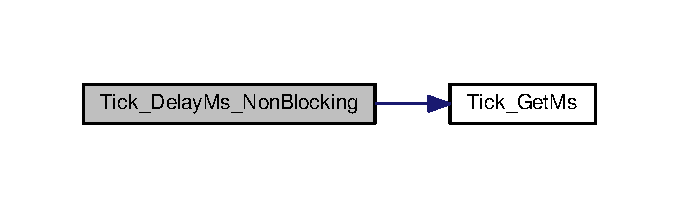
\includegraphics[width=326pt]{tick_8c_a700a086c5fb6a2a2491026af0fda77a8_cgraph}
\end{center}
\end{figure}


\hypertarget{tick_8c_a5018c28a90fe9864e870a712c8e2b571}{\index{tick.\-c@{tick.\-c}!Tick\-\_\-\-Get\-Ms@{Tick\-\_\-\-Get\-Ms}}
\index{Tick\-\_\-\-Get\-Ms@{Tick\-\_\-\-Get\-Ms}!tick.c@{tick.\-c}}
\subsubsection[{Tick\-\_\-\-Get\-Ms}]{\setlength{\rightskip}{0pt plus 5cm}uint32\-\_\-t Tick\-\_\-\-Get\-Ms (
\begin{DoxyParamCaption}
\item[{void}]{}
\end{DoxyParamCaption}
)}}\label{tick_8c_a5018c28a90fe9864e870a712c8e2b571}


return the number of mili-\/seconds since power up. 

\begin{DoxyReturn}{Returns}
number of mili-\/seconds.
\end{DoxyReturn}
\begin{DoxyNote}{Note}
the tick counter is expected to overflow and therefore code using the tick value should take this into account. 
\end{DoxyNote}


Here is the caller graph for this function\-:\nopagebreak
\begin{figure}[H]
\begin{center}
\leavevmode
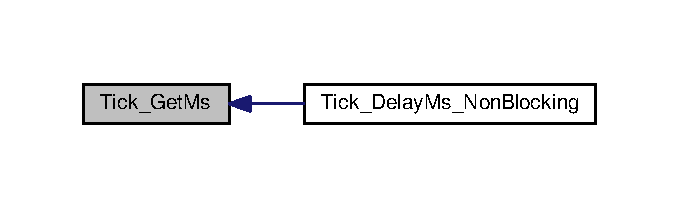
\includegraphics[width=326pt]{tick_8c_a5018c28a90fe9864e870a712c8e2b571_icgraph}
\end{center}
\end{figure}



\hypertarget{tick_8h}{\section{tick.\-h File Reference}
\label{tick_8h}\index{tick.\-h@{tick.\-h}}
}
{\ttfamily \#include \char`\"{}common.\-h\char`\"{}}\\*
Include dependency graph for tick.\-h\-:\nopagebreak
\begin{figure}[H]
\begin{center}
\leavevmode
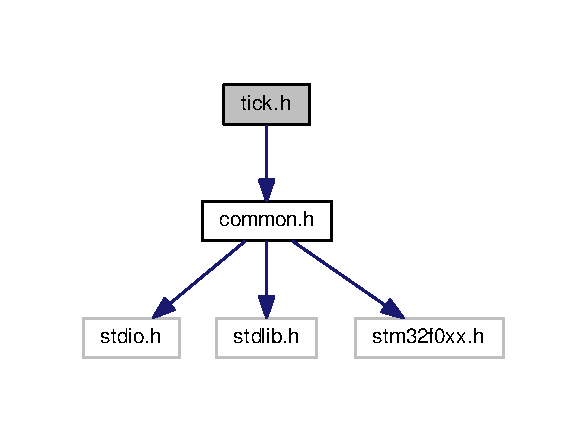
\includegraphics[width=281pt]{tick_8h__incl}
\end{center}
\end{figure}
This graph shows which files directly or indirectly include this file\-:\nopagebreak
\begin{figure}[H]
\begin{center}
\leavevmode
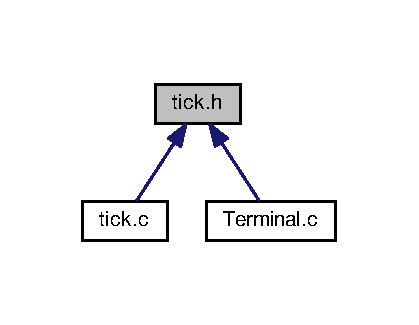
\includegraphics[width=201pt]{tick_8h__dep__incl}
\end{center}
\end{figure}
\subsection*{Classes}
\begin{DoxyCompactItemize}
\item 
struct \hyperlink{struct_tick_type}{Tick\-Type}
\begin{DoxyCompactList}\small\item\em defines a non-\/blocking delay data type. \end{DoxyCompactList}\end{DoxyCompactItemize}
\subsection*{Functions}
\begin{DoxyCompactItemize}
\item 
void \hyperlink{tick_8h_ade660961e7af4755750dd6ff81535e68}{Tick\-\_\-init} (void)
\begin{DoxyCompactList}\small\item\em setup the A\-R\-M M0 tick counter to trigger every 1ms \end{DoxyCompactList}\item 
uint32\-\_\-t \hyperlink{tick_8h_a5018c28a90fe9864e870a712c8e2b571}{Tick\-\_\-\-Get\-Ms} (void)
\begin{DoxyCompactList}\small\item\em return the number of mili-\/seconds since power up. \end{DoxyCompactList}\item 
int\-\_\-fast8\-\_\-t \hyperlink{tick_8h_a700a086c5fb6a2a2491026af0fda77a8}{Tick\-\_\-\-Delay\-Ms\-\_\-\-Non\-Blocking} (uint\-\_\-fast8\-\_\-t reset, \hyperlink{struct_tick_type}{Tick\-Type} $\ast$config)
\begin{DoxyCompactList}\small\item\em Non-\/blocking delay in ms. \end{DoxyCompactList}\item 
void \hyperlink{tick_8h_a01864fcfa99d364250b9e3e10390ff93}{Tick\-\_\-\-Delay\-Ms} (uint32\-\_\-t delay\-Ms)
\begin{DoxyCompactList}\small\item\em this is a blocking delay. \end{DoxyCompactList}\end{DoxyCompactItemize}


\subsection{Detailed Description}
Author\-: Ronald Sousa () 

\subsection{Function Documentation}
\hypertarget{tick_8h_a01864fcfa99d364250b9e3e10390ff93}{\index{tick.\-h@{tick.\-h}!Tick\-\_\-\-Delay\-Ms@{Tick\-\_\-\-Delay\-Ms}}
\index{Tick\-\_\-\-Delay\-Ms@{Tick\-\_\-\-Delay\-Ms}!tick.h@{tick.\-h}}
\subsubsection[{Tick\-\_\-\-Delay\-Ms}]{\setlength{\rightskip}{0pt plus 5cm}void Tick\-\_\-\-Delay\-Ms (
\begin{DoxyParamCaption}
\item[{uint32\-\_\-t}]{delay\-Ms}
\end{DoxyParamCaption}
)}}\label{tick_8h_a01864fcfa99d364250b9e3e10390ff93}


this is a blocking delay. 


\begin{DoxyCode}
\textcolor{preprocessor}{ #include "\hyperlink{common_8h}{common.h}"}
\textcolor{preprocessor}{ #include "\hyperlink{led_8h}{MCU/led.h}"}
\textcolor{preprocessor}{ #include "\hyperlink{tick_8h}{MCU/tick.h}"}

 \textcolor{keywordtype}{void} \hyperlink{main_8c_a6288eba0f8e8ad3ab1544ad731eb7667}{main}(\textcolor{keywordtype}{void}) \{

     \hyperlink{led_8c_af1aee968a5ceeb7915921aa6d78aca23}{Led\_Init}();
     \hyperlink{tick_8c_ade660961e7af4755750dd6ff81535e68}{Tick\_init}();

     \textcolor{keywordflow}{for}( ;;) \{
       \hyperlink{tick_8c_a01864fcfa99d364250b9e3e10390ff93}{Tick\_DelayMs}(1000); \textcolor{comment}{// delay 1s;}
       \hyperlink{led_8c_a5ebbd778fb3444fbfbded2130e08b33d}{Led\_Toggle}();
     \}
\}
\end{DoxyCode}



\begin{DoxyParams}{Parameters}
{\em delay\-Ms} & how long to delay for. \\
\hline
\end{DoxyParams}
\hypertarget{tick_8h_a700a086c5fb6a2a2491026af0fda77a8}{\index{tick.\-h@{tick.\-h}!Tick\-\_\-\-Delay\-Ms\-\_\-\-Non\-Blocking@{Tick\-\_\-\-Delay\-Ms\-\_\-\-Non\-Blocking}}
\index{Tick\-\_\-\-Delay\-Ms\-\_\-\-Non\-Blocking@{Tick\-\_\-\-Delay\-Ms\-\_\-\-Non\-Blocking}!tick.h@{tick.\-h}}
\subsubsection[{Tick\-\_\-\-Delay\-Ms\-\_\-\-Non\-Blocking}]{\setlength{\rightskip}{0pt plus 5cm}int\-\_\-fast8\-\_\-t Tick\-\_\-\-Delay\-Ms\-\_\-\-Non\-Blocking (
\begin{DoxyParamCaption}
\item[{uint\-\_\-fast8\-\_\-t}]{reset, }
\item[{{\bf Tick\-Type} $\ast$}]{config}
\end{DoxyParamCaption}
)}}\label{tick_8h_a700a086c5fb6a2a2491026af0fda77a8}


Non-\/blocking delay in ms. 


\begin{DoxyCode}
\textcolor{preprocessor}{ #include "\hyperlink{common_8h}{common.h}"}
\textcolor{preprocessor}{ #include "\hyperlink{led_8h}{MCU/led.h}"}
\textcolor{preprocessor}{ #include "\hyperlink{tick_8h}{MCU/tick.h}"}

 \textcolor{keywordtype}{void} \hyperlink{main_8c_a6288eba0f8e8ad3ab1544ad731eb7667}{main}(\textcolor{keywordtype}{void}) \{
     \hyperlink{struct_tick_type}{TickType} Delay;
     Delay.\hyperlink{struct_tick_type_ae24ecd63a2b008c5c9a6864cbb3b30a7}{DelayMs} = 1000; \textcolor{comment}{//set to 1s}

     \hyperlink{led_8c_af1aee968a5ceeb7915921aa6d78aca23}{Led\_Init}();
     \hyperlink{tick_8c_ade660961e7af4755750dd6ff81535e68}{Tick\_init}();

     \textcolor{comment}{// reset the counter}
     \hyperlink{tick_8c_a700a086c5fb6a2a2491026af0fda77a8}{Tick\_DelayMs\_NonBlocking}(\hyperlink{common_8h_aa8cecfc5c5c054d2875c03e77b7be15d}{TRUE}, &Delay);

     \textcolor{keywordflow}{for}( ;;) \{

         \textcolor{keywordflow}{if}(\hyperlink{tick_8c_a700a086c5fb6a2a2491026af0fda77a8}{Tick\_DelayMs\_NonBlocking}(\hyperlink{common_8h_aa8cecfc5c5c054d2875c03e77b7be15d}{TRUE}, &Delay)) \{
             \textcolor{comment}{// Delay has been reached}

             \hyperlink{tick_8c_a700a086c5fb6a2a2491026af0fda77a8}{Tick\_DelayMs\_NonBlocking}(\hyperlink{common_8h_aa8cecfc5c5c054d2875c03e77b7be15d}{TRUE}, &Delay);
             \hyperlink{led_8c_a5ebbd778fb3444fbfbded2130e08b33d}{Led\_Toggle}();
             \}
         \textcolor{keywordflow}{else} \{
             \textcolor{comment}{// User code when the code delay hasn't passed}
             \}

     \}
\}
\end{DoxyCode}



\begin{DoxyParams}{Parameters}
{\em reset} & true = reset timer start value/ false = Check if time has lapsed \\
\hline
{\em config} & delay setting\\
\hline
\end{DoxyParams}
\begin{DoxyReturn}{Returns}
1 = the desire delay has been reached. 0 = not reached the desire delay time. -\/1 = config point is null 
\end{DoxyReturn}


Here is the call graph for this function\-:\nopagebreak
\begin{figure}[H]
\begin{center}
\leavevmode
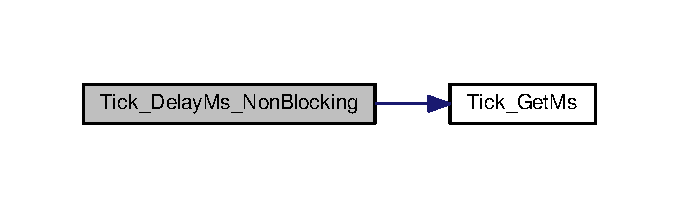
\includegraphics[width=326pt]{tick_8h_a700a086c5fb6a2a2491026af0fda77a8_cgraph}
\end{center}
\end{figure}


\hypertarget{tick_8h_a5018c28a90fe9864e870a712c8e2b571}{\index{tick.\-h@{tick.\-h}!Tick\-\_\-\-Get\-Ms@{Tick\-\_\-\-Get\-Ms}}
\index{Tick\-\_\-\-Get\-Ms@{Tick\-\_\-\-Get\-Ms}!tick.h@{tick.\-h}}
\subsubsection[{Tick\-\_\-\-Get\-Ms}]{\setlength{\rightskip}{0pt plus 5cm}uint32\-\_\-t Tick\-\_\-\-Get\-Ms (
\begin{DoxyParamCaption}
\item[{void}]{}
\end{DoxyParamCaption}
)}}\label{tick_8h_a5018c28a90fe9864e870a712c8e2b571}


return the number of mili-\/seconds since power up. 

\begin{DoxyReturn}{Returns}
number of mili-\/seconds.
\end{DoxyReturn}
\begin{DoxyNote}{Note}
the tick counter is expected to overflow and therefore code using the tick value should take this into account. 
\end{DoxyNote}


Here is the caller graph for this function\-:\nopagebreak
\begin{figure}[H]
\begin{center}
\leavevmode
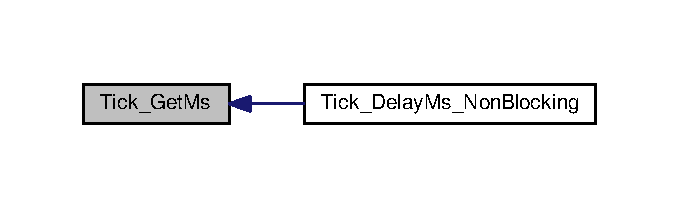
\includegraphics[width=326pt]{tick_8h_a5018c28a90fe9864e870a712c8e2b571_icgraph}
\end{center}
\end{figure}


\hypertarget{tick_8h_ade660961e7af4755750dd6ff81535e68}{\index{tick.\-h@{tick.\-h}!Tick\-\_\-init@{Tick\-\_\-init}}
\index{Tick\-\_\-init@{Tick\-\_\-init}!tick.h@{tick.\-h}}
\subsubsection[{Tick\-\_\-init}]{\setlength{\rightskip}{0pt plus 5cm}void Tick\-\_\-init (
\begin{DoxyParamCaption}
\item[{void}]{}
\end{DoxyParamCaption}
)}}\label{tick_8h_ade660961e7af4755750dd6ff81535e68}


setup the A\-R\-M M0 tick counter to trigger every 1ms 



Here is the caller graph for this function\-:
\nopagebreak
\begin{figure}[H]
\begin{center}
\leavevmode
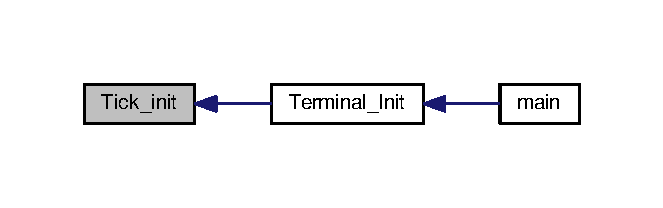
\includegraphics[width=318pt]{tick_8h_ade660961e7af4755750dd6ff81535e68_icgraph}
\end{center}
\end{figure}



\hypertarget{usart2_8c}{\section{usart2.\-c File Reference}
\label{usart2_8c}\index{usart2.\-c@{usart2.\-c}}
}


S\-T\-M32 serial2 M\-C\-U hardware interface layer. to maintain code portability, the hardware related code is split from the main logic.  


{\ttfamily \#include \char`\"{}M\-C\-U/usart2.\-h\char`\"{}}\\*
{\ttfamily \#include \char`\"{}../\-F\-I\-F\-O.\-h\char`\"{}}\\*
Include dependency graph for usart2.\-c\-:\nopagebreak
\begin{figure}[H]
\begin{center}
\leavevmode
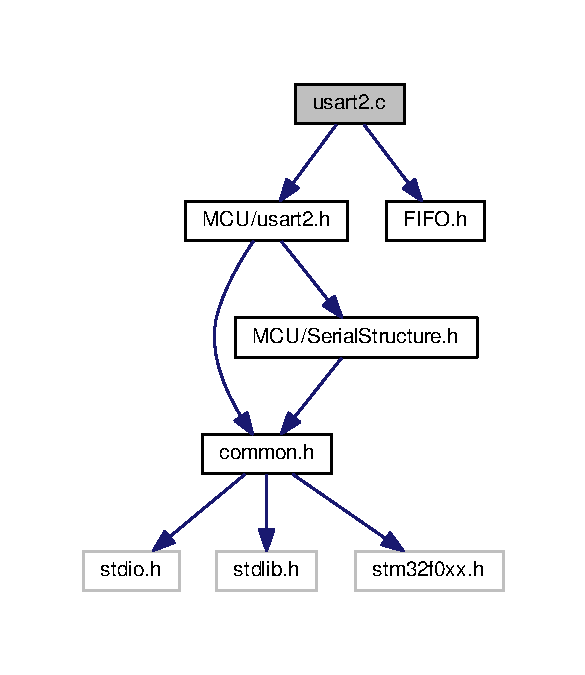
\includegraphics[width=281pt]{usart2_8c__incl}
\end{center}
\end{figure}
\subsection*{Macros}
\begin{DoxyCompactItemize}
\item 
\hypertarget{usart2_8c_a7bc0edf283b01a071b7ed8451eada11c}{\#define \hyperlink{usart2_8c_a7bc0edf283b01a071b7ed8451eada11c}{G\-P\-I\-O\-\_\-\-A\-F\-R\-L\-\_\-\-A\-F\-R2\-\_\-0}~((uint32\-\_\-t) 0x00000100)}\label{usart2_8c_a7bc0edf283b01a071b7ed8451eada11c}

\begin{DoxyCompactList}\small\item\em alternative function set bit 1 for A\-F\-R2 \end{DoxyCompactList}\item 
\hypertarget{usart2_8c_af91c2a8b8c966e16328c4384d1a31b23}{\#define \hyperlink{usart2_8c_af91c2a8b8c966e16328c4384d1a31b23}{G\-P\-I\-O\-\_\-\-A\-F\-R\-L\-\_\-\-A\-F\-R3\-\_\-0}~((uint32\-\_\-t) 0x00001000)}\label{usart2_8c_af91c2a8b8c966e16328c4384d1a31b23}

\begin{DoxyCompactList}\small\item\em alternative function set bit 1 for A\-F\-R3 \end{DoxyCompactList}\end{DoxyCompactItemize}
\subsection*{Functions}
\begin{DoxyCompactItemize}
\item 
void \hyperlink{usart2_8c_a0ca6fd0e6f77921dd1123539857ba0a8}{U\-S\-A\-R\-T2\-\_\-\-I\-R\-Q\-Handler} (void)
\begin{DoxyCompactList}\small\item\em the U\-S\-A\-R\-T 2 interrupt handler. \end{DoxyCompactList}\end{DoxyCompactItemize}
\subsection*{Variables}
\begin{DoxyCompactItemize}
\item 
\hyperlink{struct_serial_interface}{Serial\-Interface} \hyperlink{usart2_8c_a0ad9cd4fbffc7497abd537641dcc99af}{Serial\-Port2}
\begin{DoxyCompactList}\small\item\em Defines the standard serial functions for usart 2. \end{DoxyCompactList}\end{DoxyCompactItemize}


\subsection{Detailed Description}
S\-T\-M32 serial2 M\-C\-U hardware interface layer. to maintain code portability, the hardware related code is split from the main logic. Author\-: Ronald Sousa (Opticalworm) 

\subsection{Function Documentation}
\hypertarget{usart2_8c_a0ca6fd0e6f77921dd1123539857ba0a8}{\index{usart2.\-c@{usart2.\-c}!U\-S\-A\-R\-T2\-\_\-\-I\-R\-Q\-Handler@{U\-S\-A\-R\-T2\-\_\-\-I\-R\-Q\-Handler}}
\index{U\-S\-A\-R\-T2\-\_\-\-I\-R\-Q\-Handler@{U\-S\-A\-R\-T2\-\_\-\-I\-R\-Q\-Handler}!usart2.c@{usart2.\-c}}
\subsubsection[{U\-S\-A\-R\-T2\-\_\-\-I\-R\-Q\-Handler}]{\setlength{\rightskip}{0pt plus 5cm}void U\-S\-A\-R\-T2\-\_\-\-I\-R\-Q\-Handler (
\begin{DoxyParamCaption}
\item[{void}]{}
\end{DoxyParamCaption}
)}}\label{usart2_8c_a0ca6fd0e6f77921dd1123539857ba0a8}


the U\-S\-A\-R\-T 2 interrupt handler. 

\begin{DoxyRefDesc}{Todo}
\item[\hyperlink{todo__todo000002}{Todo}]Need to implement the T\-X interrupt \end{DoxyRefDesc}


\subsection{Variable Documentation}
\hypertarget{usart2_8c_a0ad9cd4fbffc7497abd537641dcc99af}{\index{usart2.\-c@{usart2.\-c}!Serial\-Port2@{Serial\-Port2}}
\index{Serial\-Port2@{Serial\-Port2}!usart2.c@{usart2.\-c}}
\subsubsection[{Serial\-Port2}]{\setlength{\rightskip}{0pt plus 5cm}{\bf Serial\-Interface} Serial\-Port2}}\label{usart2_8c_a0ad9cd4fbffc7497abd537641dcc99af}
{\bfseries Initial value\-:}
\begin{DoxyCode}
= \{
                                    IsSerialOpen,
                                    Open,
                                    Close,
                                    SendByte,
                                    SendString,
                                    SendArray,
                                    DoesReceiveBufferHaveData,
                                    GetByte
                                \}
\end{DoxyCode}


Defines the standard serial functions for usart 2. 

\begin{DoxySeeAlso}{See Also}
\hyperlink{struct_serial_interface}{Serial\-Interface} 
\end{DoxySeeAlso}

\hypertarget{usart2_8h}{\section{usart2.\-h File Reference}
\label{usart2_8h}\index{usart2.\-h@{usart2.\-h}}
}
{\ttfamily \#include \char`\"{}common.\-h\char`\"{}}\\*
{\ttfamily \#include \char`\"{}M\-C\-U/\-Serial\-Structure.\-h\char`\"{}}\\*
Include dependency graph for usart2.\-h\-:\nopagebreak
\begin{figure}[H]
\begin{center}
\leavevmode
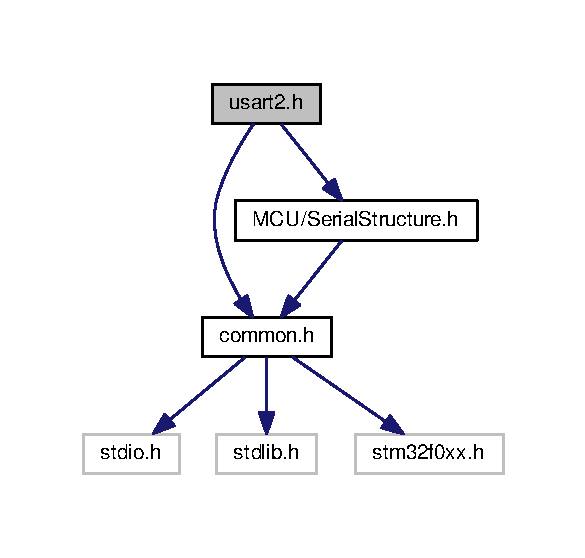
\includegraphics[width=281pt]{usart2_8h__incl}
\end{center}
\end{figure}
This graph shows which files directly or indirectly include this file\-:\nopagebreak
\begin{figure}[H]
\begin{center}
\leavevmode
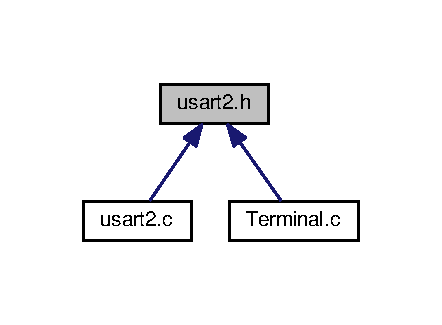
\includegraphics[width=196pt]{usart2_8h__dep__incl}
\end{center}
\end{figure}
\subsection*{Variables}
\begin{DoxyCompactItemize}
\item 
\hyperlink{struct_serial_interface}{Serial\-Interface} \hyperlink{usart2_8h_a0ad9cd4fbffc7497abd537641dcc99af}{Serial\-Port2}
\begin{DoxyCompactList}\small\item\em Defines the standard serial functions for usart 2. \end{DoxyCompactList}\end{DoxyCompactItemize}


\subsection{Detailed Description}
Author\-: Ronald Sousa () 

\subsection{Variable Documentation}
\hypertarget{usart2_8h_a0ad9cd4fbffc7497abd537641dcc99af}{\index{usart2.\-h@{usart2.\-h}!Serial\-Port2@{Serial\-Port2}}
\index{Serial\-Port2@{Serial\-Port2}!usart2.h@{usart2.\-h}}
\subsubsection[{Serial\-Port2}]{\setlength{\rightskip}{0pt plus 5cm}{\bf Serial\-Interface} Serial\-Port2}}\label{usart2_8h_a0ad9cd4fbffc7497abd537641dcc99af}


Defines the standard serial functions for usart 2. 

\begin{DoxySeeAlso}{See Also}
\hyperlink{struct_serial_interface}{Serial\-Interface} 
\end{DoxySeeAlso}

%--- End generated contents ---

% Index
\newpage
\phantomsection
\addcontentsline{toc}{chapter}{Index}
\printindex

\end{document}
